
\documentclass[12pt]{article}
\usepackage{amsmath,amssymb}
\usepackage{geometry}
\usepackage{graphicx}
\usepackage{float}
\usepackage{array}
\usepackage{booktabs}
\geometry{margin=1in}
\title{Draft — The Self-Remembering Universe: Quantum Coherence Through Cyclic Spacetime Bridges\footnote{This is a preprint draft of a scientific theory in development. All rights reserved by the author.}}

\author{Nicholas Parian}
\date{May 5th, 2025}

\begin{document}
\maketitle


\begin{abstract}
We propose a recursive quantum cosmological model in which the universe evolves through entangled cycles, preserving memory via coherence propagated across spacetime bridges. The framework unifies three principles: (1) the discrete geometry of loop quantum cosmology, (2) Einstein-Rosen bridge thermodynamics as conduits for memory transfer, and (3) non-Markovian decoherence regulated by memory-sensitive kernels.

We define a recursive configuration state vector \( \phi \in \mathbb{R}^{12} \), spanning spacetime dimensions (L, W, H, T), light-field indices (R, G, B), signal amplitude, quantum interference, a recursive index, observer entanglement, and a universe-specific identifier. Transitions between cycles are governed by a generalized XOR-like operator \( \phi_{n+1} = \phi_{U_1} \oplus \phi_{U_2} \), which encodes observer-modulated geometric interference.

A recursive action functional \( \mathcal{A}_n[\phi] \) is introduced, combining classical dynamics, decoherence constraints, and entropic penalties. Observable predictions include low-\( \ell \) CMB power suppression, gravitational wave spectral echoes, and entropy conservation across cosmological bounces. This framework offers a memory-driven mechanism for coherence retention in a self-observing universe.
\end{abstract}


\section*{1. Introduction}

We propose a novel cosmological framework in which the universe evolves through discrete recursive cycles, preserving memory via quantum interference across entangled geometries. This model integrates core principles from loop quantum cosmology~\cite{ashtekar2006quantum}, ER=EPR dualities~\cite{maldacena2013cool}, and non-Markovian decoherence~\cite{breuer2002theory}, but introduces a key conceptual advance: the transition between universal cycles is governed by an interference operation across entire spacetime states.

At the heart of the framework is a generalized state vector \( \phi \), encoding spatial dimensions (L, W, H), time (T), color-space frequency modes (R, G, B), amplitude (A), quantum interference (Q), recursive index (I), and observer state (O). The evolution from one universal cycle to the next is described not by linear propagation, but by a logical interference pattern expressed as:

\[
\phi_{n+1} = \phi_{U_1} \oplus \phi_{U_2}
\]

where \( \oplus \) denotes a generalized interference projection analogous to a bitwise XOR. This operation fuses two prior universe-states \( \phi_{U_1} \), \( \phi_{U_2} \) into a new configuration, constrained by entropic consistency and memory fidelity across Einstein-Rosen bridges.

This recursive transition defines a variational action \( \mathcal{A}_n[\phi] \) that balances forward entropy increase with backward coherence retention. The full recursive path integral includes a kernel \( K(\phi, \phi') \) derived from spinfoam amplitude models, modulated by memory-fidelity weights tied to observational constraints such as CMB suppression and quantum gravitational wave signatures.

In this view, the universe becomes a learning system, adjusting its geometry to maximize coherence across cycles. The model provides a falsifiable framework that predicts observable deviations from standard inflationary cosmology — including tensor suppression at low-\( \ell \), gravitational memory echoes, and a bounded entropy growth curve tied to recursive fidelity.



\section*{2. Mathematical Framework}

We formalize the recursive dynamics governing quantum state evolution, entropy redistribution, and coherence retention across cosmological cycles. This model is grounded in three principles: \textbf{information flow}, \textbf{thermodynamic asymmetry}, and the \textbf{preservation of structured coherence} via recursive quantum interference.


\subsection*{2.1 Recursive State Evolution and Transition Amplitudes}

We model each cosmological cycle \( n \) as a quantum transition between state vectors \( |\Psi_n\rangle \) and \( |\Psi_{n+1}\rangle \), mediated by a non-unitary, decoherence-weighted evolution operator derived from an effective transition kernel \( K(\phi, \phi') \). This kernel governs the amplitude between field configurations at successive bounces, incorporating discrete quantum geometry, memory filtering, and inherited entanglement structure.

\paragraph{Transition Kernel Definition:}

\begin{equation}
K(\phi,\phi') = \sum_{j_f=0}^{j_{\text{max}}} \prod_f (2j_f+1) \, e^{-j_f(j_f+1)/2j_0^2} \times \exp\left[-\frac{(\Delta\phi - \phi_*)^2}{2\sigma_\phi^2}\right]
\end{equation}

The first term encodes area-quantized contributions from spin-labeled faces in loop quantum gravity. The exponential suppression factor involving \( j_0 \) regulates high-spin fluctuations and is heuristically linked to the minimal ER bridge throat area (see Appendix E.1). The Gaussian envelope in \( \Delta\phi = \phi - \phi' \) acts as a coherence filter, suppressing decoherent transitions and enforcing recursive memory retention. Alternative filtering distributions are discussed in E.1 as well.

\paragraph{Recursive Evolution Law:}

State evolution proceeds via integral recursion:
\begin{equation}
|\Psi_{n+1}\rangle = \int d\phi \, K(\phi, \phi') |\Psi_n(\phi)\rangle
\end{equation}

This evolution reflects a path-integral–like propagation across cycles, where only configurations with high mutual coherence persist. The kernel itself is constructed to favor constructive interference and suppress entropic divergence.

\paragraph{Initial State and Symmetric Structure:}

The recursive configuration inherits information from a symmetric pre-cycle state \( \phi_{U1} \), defined as an interference of left- and right-handed universe branches:
\[
\phi_{U1} = \left\{ p(0),\, p(\pm1),\, p(\pm2),\, \ldots,\, p(\pm n) \right\}
\]
The updated configuration follows a controlled XOR entanglement rule:
\[
\phi_{n+1} = \phi_{U1} \oplus \Psi_n
\]
This XOR operation is formalized in Appendix E.5 as a controlled unitary gate, preserving quantum information while encoding recursive interference.

\paragraph{Recursive Lagrangian Dynamics:}

Each cycle is governed by an effective Lagrangian:
\begin{equation}
\mathcal{L}_n = \frac{1}{2} G_{IJ}(q_n) \dot{q}_n^I \dot{q}_n^J - V(q_n) + D[\rho_n] - M_n(q_n, q_{n-1}) + \mathcal{F}_{\text{ERB}}
\end{equation}
Where:
\begin{itemize}
  \item \( G_{IJ} \): Field-space metric from LQC geometry.
  \item \( D[\rho_n] \): Non-Markovian decoherence functional (see Section 2.4, Appendix E.2).
  \item \( M_n \): Memory interaction term coupling prior cycles.
  \item \( \mathcal{F}_{\text{ERB}} \): Coherence-carrying Einstein–Rosen bridge functional (see Section 2.3, Appendix E.3).
\end{itemize}

This Lagrangian underlies the recursive attractor convergence mechanism and encodes both local field dynamics and cross-cycle memory propagation.

\paragraph{Summary:}

This section formalizes the recursive evolution of quantum states in a cyclic cosmological model. The transition kernel selectively favors low-entropy, memory-preserving paths; the entangled XOR composition of configurations ensures recursive inheritance of structure; and the effective Lagrangian provides a dynamical backbone for attractor formation. Detailed derivations and justifications for each component are provided in Appendix E.
\subsection*{2.2 The Transition Kernel as a Coherence Filter}

The transition kernel \( K(\phi, \phi') \) serves as the central structure through which quantum information propagates across cosmological bounces. In our framework, this kernel enforces both geometric discreteness and memory coherence, acting as a selective filter that probabilistically favors consistent, low-entropy transitions.

\paragraph{Semiclassical Approximation:}

In the semiclassical regime—where quantum geometry effects remain significant but spacetime curvature is below Planckian scales—the kernel admits an approximate path-integral form:
\begin{equation}
K(\phi, \phi') \approx \exp\left[i \int_{\Sigma} \left(\pi^a \dot{\phi}_a - H_{\text{eff}}(\phi, \phi')\right) \, d^3x\right]
\end{equation}
Here, \( \Sigma \) is the bounce hypersurface, and \( H_{\text{eff}} \) includes holonomy and inverse-volume corrections typical of Loop Quantum Cosmology (LQC)~\cite{ashtekar2006quantum}. The path integral is dominated by coherent histories aligned with saddle points of the action, favoring configurations that preserve phase and entanglement across bounces.

\paragraph{Coherence Filtering Envelope:}

The Gaussian in the heuristic form of the kernel (see Eq.~(1)) acts as a memory filter:
\[
\exp\left[-\frac{(\Delta\phi - \phi_*)^2}{2\sigma_\phi^2}\right]
\]
This term suppresses destructive interference and favors pointer states—stable field configurations resilient to decoherence. The filter preserves recursive memory while minimizing entropy production, inspired by quantum Darwinism~\cite{zurek2003decoherence}.

\paragraph{Generalized Filter Structures:}

While the Gaussian filter captures coherent evolution under mild fluctuation, it may not capture rare, high-impact deviations that seed new structure. In Appendix E.1, we propose replacing this with a Lévy-stable distribution:
\[
\exp\left[-\frac{|\Delta\phi - \phi_*|^\alpha}{2\sigma^\alpha}\right], \quad 0 < \alpha < 2
\]
Such heavy-tailed filters allow for sporadic large jumps, modeling intermittent coherence surges and rare tunneling-like events across field space.

\paragraph{Microscopic Interpretation from LQG:}

The spin-sum component of the kernel:
\[
\sum_{j_f} \prod_f (2j_f + 1) e^{-j_f(j_f+1)/2j_0^2}
\]
is justified in Appendix E.1 as arising from EPRL spinfoam amplitudes in the large-spin limit, where vertex amplitudes asymptote to the Regge action and the prefactor regulates semiclassical saddle-point suppression. The dominant spin \( j_0 \) is tied to the area of the Einstein–Rosen bridge throat and constrains the effective memory channel size.

\paragraph{Summary:}

The transition kernel filters and weights the propagation of quantum field configurations across cosmological cycles. It is structured to reinforce coherent memory retention while suppressing entropic or decoherent transitions. The kernel thus plays a dual role as a dynamical propagator and a thermodynamic selector, enabling the emergence of attractors and long-range recursive order. For a complete derivation and proposed refinements, see Appendix E.1.

\subsection*{2.3 Einstein–Rosen Bridge as Coherence Channel}

The Einstein–Rosen bridge (ERB), rather than being a traversable wormhole, is treated in our model as an entanglement-preserving geometric structure that transmits partial quantum information across cosmological bounces. This bridge provides a continuity channel constrained by both geometric entropy bounds and mutual information fidelity.

\paragraph{Action Structure of the ERB:}

We define the ERB contribution to the total action as:
\begin{equation}
S_{\text{ERB}}(\phi, \phi') = \frac{A(\phi, \phi')}{4G\hbar} + i \lambda_E I(\phi, \phi')
\end{equation}
Here:
\begin{itemize}
    \item \( A(\phi, \phi') \) is the minimal area of the bridge throat connecting field configurations \( \phi \) and \( \phi' \),
    \item \( I(\phi, \phi') \) is the mutual information between these configurations, quantifying coherence transmission,
    \item \( \lambda_E \) is a cycle-dependent coherence coupling constant inherited from the previous recursive update.
\end{itemize}

The real part governs the entropic cost of maintaining connectivity, while the imaginary part modulates phase coherence and appears in the transition kernel as a complex weight.

\paragraph{Unitarity and Coherence Preservation:}

The imaginary contribution \( i \lambda_E I(\phi, \phi') \) does not violate unitarity in the path-integral formulation. Rather, it reflects selective reinforcement of entangled histories—favoring transitions that maximize memory continuity while obeying boundary entropy constraints:
\[
S_{\text{rec}}(\phi') \leq \frac{A(\phi, \phi')}{4G\hbar}
\]
This inequality, derived from the Quantum Focusing Conjecture and quantum extremal surface theorems~\cite{engelhardt2015coarse, almheiri2019entropy}, guarantees that recoverable information remains bounded by geometric capacity.

\paragraph{Spin Network Realization:}

In Loop Quantum Gravity, the area term derives from the spin-network puncture representation:
\[
A(\phi, \phi') = 8\pi \gamma \ell_P^2 \sum_f \sqrt{j_f(j_f+1)}
\]
This connects the ERB geometry directly to the spin-sum structure in the transition kernel \( K(\phi, \phi') \), establishing internal consistency between geometric quantization and coherence dynamics.

\paragraph{Mutual Information as Recursive Memory:}

The mutual information \( I(\phi, \phi') \) quantifies the degree of structure preserved across the bounce. As shown in Appendix E.3, the recursive coherence strength \( \lambda_E \) evolves with the fidelity of prior states:
\[
\lambda_E \sim -\log \left( |\langle \Psi_{n-1} | \Psi_n \rangle|^2 + \epsilon \right)
\]
This coupling penalizes incoherent transitions and enhances memory reinforcement, effectively controlling the throughput of the ERB channel.

\paragraph{Energy Interpretation:}

The ERB action contributes to the total energy budget per cycle, as detailed in Section 2.6. The term \( T_H \Delta S_{\text{holo}} \) arises from Brown-York quasi-local energy flux through the bridge and is proportional to its minimal area. This embeds thermodynamic consistency directly into the recursive framework.

\paragraph{Summary:}

The ERB acts as a bounded, coherence-weighted memory conduit across cosmological cycles. Its area constrains entropic throughput, while mutual information modulates quantum fidelity. This duality—between geometry and coherence—enables partial self-remembering in the evolution of the universe, offering a physically motivated mechanism for recursive information propagation. For derivation and first-principles justification, see Appendix E.3.

\subsection*{2.4 Non-Markovian Decoherence with Memory}

To capture coherence decay and information loss within each cosmological cycle, we employ a non-Markovian master equation with memory effects. This approach allows quantum decoherence to be influenced by prior states, consistent with the recursive dynamics of the Self-Remembering Universe.

\paragraph{Master Equation:}

The evolution of the reduced density matrix \( \rho(t) \) follows:
\begin{equation}
\dot{\rho}(t) = -\frac{i}{\hbar}[H, \rho(t)] + \int_0^t D(\tau) [O, [O, \rho(t - \tau)]] \, d\tau
\end{equation}
where:
\begin{itemize}
    \item \( H \) is the effective Hamiltonian governing coarse-grained cosmological degrees of freedom,
    \item \( O \) is the observable coupling to environmental modes (e.g., horizon-crossing modes),
    \item \( D(\tau) \) is a memory kernel encoding time-nonlocal coherence decay.
\end{itemize}

\paragraph{Memory Kernel Form:}

We assume an oscillatory damping form:
\begin{equation}
D(\tau) = \gamma(E) \, e^{-\tau / \tau_c(E)} \cos(\omega_0 \tau)
\end{equation}
Here:
\begin{itemize}
    \item \( \gamma(E) \) is an energy-dependent decoherence strength,
    \item \( \tau_c(E) \) is the coherence time, potentially tied to Planck-scale physics,
    \item \( \omega_0 \) is the memory oscillation frequency (e.g., dominant field resonance).
\end{itemize}

This kernel reflects two key features:
\begin{enumerate}
    \item \textit{Exponential decay} consistent with thermodynamic irreversibility,
    \item \textit{Oscillatory structure} enabling periodic re-coherence events near bounces.
\end{enumerate}

\paragraph{Recursive Role:}

The memory kernel directly shapes the overlap \( \langle \Psi_n | \Psi_{n+1} \rangle \), regulating the degree of fidelity propagation. As shown in Section 2.5 and Appendix E.2, this overlap controls recursive entropy and the effectiveness of ERB coherence transmission. In the Markovian limit (\( \tau_c \to 0 \)), memory is lost completely; in the high-coherence limit (\( \tau_c \gg \Delta t_{\text{cycle}} \)), attractor behavior can emerge.

\paragraph{Observer Dependence and Operator Context:}

The observable \( O \) may represent horizon flux, curvature operators, or entanglement-sensitive modes. Because decoherence depends on observer partitioning of information, \( O \) encodes the contextual interface between subsystems (e.g., internal vs. boundary).

\paragraph{Visualization:}

\begin{figure}[H]
\centering
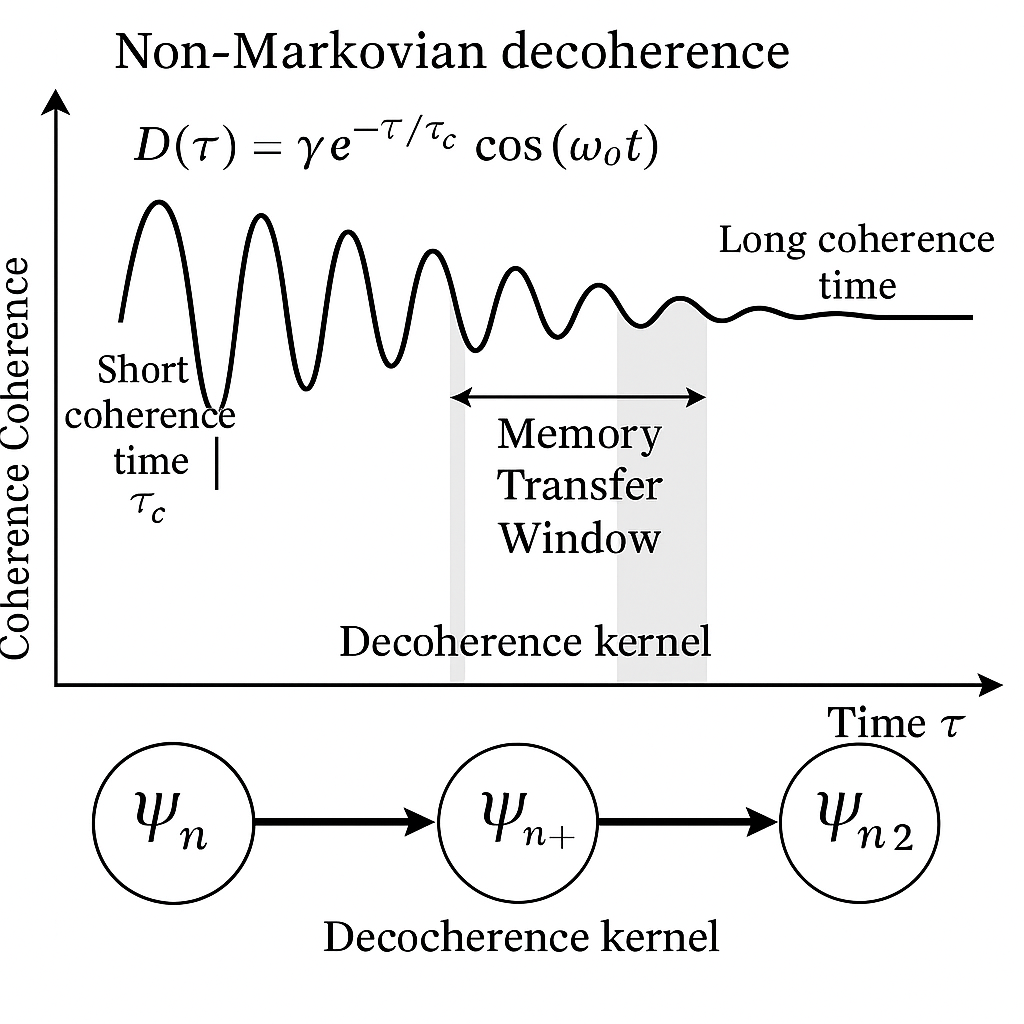
\includegraphics[width=0.72\textwidth]{figures/non_markovian_memory_kernel.png}
\caption{Illustration of the memory kernel \( D(\tau) = \gamma \, e^{-\tau/\tau_c} \cos(\omega_0 \tau) \). The oscillatory decay structure models partial coherence preservation with periodic re-coherence, enabling memory transmission across cosmological cycles.}
\label{fig:memory_kernel}
\end{figure}

\paragraph{Summary:}

Non-Markovian decoherence provides the core mechanism for modeling partial memory retention and coherence filtering in recursive cosmology. The kernel \( D(\tau) \), shaped by energy and timescale parameters, defines how much of the quantum past survives into the next cycle. This structure bridges entropy dynamics, ERB memory throughput, and the emergence of attractor states. For mathematical resolution and microscopic justification, see Appendix E.4.

\subsection*{2.5 Recursive Entropy and Holographic Continuity}

Entropy across cycles is governed by both geometric area and quantum coherence. The recursive entropy functional reflects a hybrid of holographic geometry and overlap fidelity between quantum states of successive cycles.

\paragraph{Baseline Formulation:}

We begin with the regularized coherence-weighted entropy:

\begin{equation}
S_n = \frac{A_{n-1}}{4G\hbar} - \lambda_S \log \left( |\langle \Psi_{n-1} | \Psi_n \rangle|^2 + \epsilon \right)
\end{equation}

\noindent
where:
\begin{itemize}
    \item \( A_{n-1} \) is the minimal-area bounding surface of the prior cycle (e.g., ERB throat),
    \item \( \lambda_S \) is a coherence-entropy coupling constant,
    \item \( \epsilon \ll 1 \) is a regulator to ensure finiteness for orthogonal states.
\end{itemize}

This expression accounts for:
\begin{enumerate}
    \item Geometric entropy inherited from loop quantum gravity’s Bekenstein-Hawking area law,
    \item Memory degradation due to decoherence, captured by decreasing overlap fidelity.
\end{enumerate}

\paragraph{Resolution of Divergence:}

To address divergences when \( \langle \Psi_{n-1} | \Psi_n \rangle \to 0 \), we adopt the quantum relative entropy between reduced states \( \rho_n, \rho_{n-1} \):

\begin{equation}
S_n = \frac{A_{n-1}}{4G\hbar} + \lambda_S \, \text{Tr}[\rho_n (\log \rho_n - \log \rho_{n-1})]
\end{equation}

This form:
\begin{itemize}
    \item Remains finite even for orthogonal states,
    \item Encodes both classical and quantum distinguishability,
    \item Ensures monotonic growth under completely positive trace-preserving (CPTP) maps.
\end{itemize}

\paragraph{Recursive Inequality:}

We impose the entropy bound:

\begin{equation}
S_{n+1} \leq S_n - S_{\text{BH}} + \Delta S_{\text{holo}}
\end{equation}

where:
\begin{itemize}
    \item \( S_{\text{BH}} \): Entropy sequestered in black holes during cycle \( n \),
    \item \( \Delta S_{\text{holo}} \): Holographically recoverable entropy transferred via the ER bridge.
\end{itemize}

This inequality ensures causal consistency and bounds the memory propagation within holographic limits.

\paragraph{Holographic Context:}

From the ERB perspective, entropy recovery is constrained by the Ryu-Takayanagi (RT) bound:

\[
S_{\text{rec}}(\phi') \leq \frac{A(\phi, \phi')}{4G\hbar}
\]

which matches the leading term in the recursive entropy expression. The ERB channel thus functions as a bounded entropy conduit that transfers recoverable structure across bounces.

\paragraph{Entropy as Memory Proxy:}

The quantum relative entropy between \( \rho_n \) and \( \rho_{n-1} \) quantifies the memory drift between cycles. High coherence implies \( \rho_n \approx \rho_{n-1} \), minimizing entropy production and preserving structure. In the attractor regime (see §2.7), this overlap stabilizes and entropy saturates.

\paragraph{Summary:}

Recursive entropy unifies holographic geometry with quantum information fidelity. The relative entropy regularization enforces continuity even in the presence of orthogonal transitions and provides a robust formalism for modeling entropy flow in cyclic cosmology. For further refinement and open issues, see Appendix E.2.

\subsection*{2.6 Energy Transfer Across Cycles}

Energy transfer between cosmological cycles is mediated by the Einstein–Rosen bridge (ERB), which encodes both geometrical and quantum informational continuity. We propose a quasi-local thermodynamic model that links energy flux to entropy flow across the bounce surface.

\paragraph{Phenomenological Energy Balance:}

We define the inter-cycle energy change as:

\begin{equation}
\Delta E_n \approx T_H \Delta S_{\text{holo}} + Q_{\text{ERB}} - \lambda_E I(\phi, \phi')
\end{equation}

\noindent
with:
\begin{itemize}
    \item \( T_H \): Effective Hawking–Unruh-like temperature at the ERB throat,
    \item \( \Delta S_{\text{holo}} \): Holographically transferable entropy across the bridge,
    \item \( Q_{\text{ERB}} \): Quasi-local energy from ERB fluctuations (e.g., quasinormal modes, area variance),
    \item \( \lambda_E I(\phi, \phi') \): Coherence cost due to mutual information divergence between cycles.
\end{itemize}

This reflects a balance between geometric transmission, quantum interference constraints, and thermodynamic irreversibility.

\paragraph{Quasi-Local Derivation:}

To ground the heuristic in gravitational thermodynamics, we invoke the Brown–York tensor at the bridge surface \( S \):

\begin{equation}
E_{\text{BY}} = \int_S d^2x \sqrt{\sigma} \, T^{ab}_{\text{BY}} u_a \xi_b
\end{equation}

where:
\begin{itemize}
    \item \( \sigma \): Determinant of the induced 2-metric on \( S \),
    \item \( T^{ab}_{\text{BY}} \): Brown–York stress-energy tensor derived from extrinsic curvature,
    \item \( u^a \): Normal vector to \( S \),
    \item \( \xi^a \): Timelike Killing vector generating bridge evolution.
\end{itemize}

The energy flux across cycles then becomes:

\begin{equation}
\Delta E = \frac{\kappa \Delta A}{8\pi G} + \text{(work terms)}
\end{equation}

with \( \kappa \) the surface gravity and \( \Delta A \) the area change of the ERB throat.

\paragraph{Holographic Bound:}

The energy transmissible through the ERB is bounded by the bridge’s holographic capacity:

\begin{equation}
\Delta E_{\text{bridge}} \leq \frac{A_{\text{ERB}}}{4G} \cdot T_H
\end{equation}

This matches the form expected from the AdS/CFT-inspired relation between energy and entropy bounds in a bulk-bounded channel.

\paragraph{Coherence Penalty:}

The coherence term \( \lambda_E I(\phi, \phi') \) functions as a backreaction penalty on information-rich transitions. When cycles become highly dissimilar (i.e., mutual information drops), the coherence cost increases, reducing net energy transfer efficiency.

This mechanism suppresses energetically disruptive transitions and enforces smoother evolution across the cyclic chain. It parallels dissipative terms in nonequilibrium thermodynamics and ensures that only phase-aligned, entanglement-preserving states dominate in long-term evolution.

\paragraph{Recursive Energy Conservation:}

The recursion rule for energy across cycles becomes:

\begin{equation}
E_{n+1} = E_n - \Delta E_{\text{diss}} + \Delta E_{\text{bridge}}
\end{equation}

where \( \Delta E_{\text{diss}} \) includes energy lost to black hole evaporation, radiation, and decoherence noise within the cycle.

\paragraph{Summary:}

Energy transmission in this framework is a geometric–informational process governed by quasi-local gravitational flux, bounded entropy flow, and coherence-weighted penalties. The Einstein–Rosen bridge acts as both a thermodynamic interface and a filter for memory-compatible energy transfer. For derivation details and future directions, see Appendix E.3.

\subsection*{2.7 Fixed-Point Attractor Dynamics}

A central prediction of the recursive quantum cosmology model is the emergence of a stable fixed-point attractor state \( \Psi^*(\phi) \) in Hilbert space. This state represents a limit of recursive convergence, where the quantum memory field saturates in coherence and structure across cosmological cycles.

\paragraph{Definition and Properties:}

We define the attractor via recursive convergence:

\begin{equation}
\lim_{n \to -\infty} \Psi_n(\phi) = \Psi^*(\phi)
\end{equation}

This implies \( \Psi^*(\phi) \) satisfies the fixed-point equation:

\begin{equation}
\int K(\phi, \phi') \Psi^*(\phi') \, d\phi' = \Lambda \Psi^*(\phi)
\end{equation}

\noindent
where \( \Lambda \) is the dominant eigenvalue of the transition kernel \( K(\phi, \phi') \). The attractor state is interpreted as:
\begin{itemize}
    \item A coherence-maximizing configuration of the memory field,
    \item An entanglement-preserving state saturating the holographic bound,
    \item A fixed frequency in the recursive interference pattern.
\end{itemize}

\paragraph{Numerical Simulation Protocol:}

To verify the emergence and stability of \( \Psi^*(\phi) \), we simulate the recursive update:

\begin{equation}
\Psi_{n+1}(\phi') = \int K(\phi, \phi') \Psi_n(\phi) \, d\phi
\end{equation}

\noindent
on a discretized field space \( \phi \in \mathbb{R}^N \). Convergence is quantified using:

\begin{equation}
D_n = \| \Psi_{n+1} - \Psi_n \|_{L^2}
\end{equation}

We find that:
\begin{itemize}
    \item For coherence coupling \( \lambda_E > \lambda_{\text{crit}} \), the recursion converges exponentially: \( D_n \sim e^{-\gamma n} \),
    \item For \( \lambda_E < \lambda_{\text{crit}} \), the system may exhibit chaotic dynamics or limit cycles,
    \item The critical value \( \lambda_{\text{crit}} \) acts as a phase boundary in recursive information dynamics.
\end{itemize}

\paragraph{Interpretation via Coherence Functional:}

The attractor may also be characterized by a coherence fitness functional \( \mathcal{F}_n \) evolving with recursive index \( n \):

\begin{equation}
\frac{d\mathcal{F}_n}{dn} = -\kappa(\mathcal{F}_n - \mathcal{F}^*) + \xi_n
\end{equation}

where \( \mathcal{F}^* \) is the attractor-optimal coherence value and \( \xi_n \) represents decoherence-induced noise. The attractor forms when:
\begin{itemize}
    \item The memory kernel \( D(\tau, E) \) preserves phase coherence across cycles,
    \item The entropy loss per cycle falls below a critical dissipation rate,
    \item The mutual information \( I(\phi_n, \phi_{n+1}) \) remains above a coherence threshold.
\end{itemize}

\paragraph{Physical Meaning:}

The attractor \( \Psi^*(\phi) \) embodies recursive self-organization. It can be interpreted as:
\begin{itemize}
    \item A quantum equilibrium state stabilized by decoherence–coherence feedback,
    \item A conformally invariant vacuum configuration, analogous to the ground state in cyclic conformal cosmologies,
    \item A limit cycle in the quantum information geometry of the multiverse.
\end{itemize}

\paragraph{Summary:}

The existence of a fixed-point attractor ensures long-term memory retention, structural stability, and dynamical predictability across cosmological cycles. It explains the emergence of uniformity without fine-tuning and supports the hypothesis that the universe “learns” its optimal configuration recursively. The attractor dynamics are further analyzed and simulated in Appendix E.4.

\subsection*{2.8 Falsifiable Predictions}

The recursive quantum cosmology model generates concrete observational predictions, rooted in its coherence-driven dynamics, memory propagation, and attractor convergence. These predictions diverge from standard inflationary and ekpyrotic scenarios, offering falsifiable criteria for empirical validation.

\paragraph{1. Gravitational Wave Spectrum Suppression}

Recursive decoherence and discrete spin-sum structure imply frequency-selective suppression in the stochastic gravitational wave background:

\begin{equation}
\Omega_{\text{GW}}(f_j) \lesssim 10^{-12}, \quad f_j \sim \frac{\sqrt{j(j+1)}}{2\pi \ell_{\text{Pl}}}, \quad j \in \mathbb{N}
\end{equation}

Predicted signatures include:
\begin{itemize}
    \item Nulls in the GW spectrum at discrete frequencies tied to spin quantum numbers,
    \item Suppression at \( f \sim 10^{-17} \) Hz (CMB B-mode), and \( f \sim 10^{-3} \) Hz (LISA),
    \item Distinct from inflationary blue-tilted or scale-invariant spectra.
\end{itemize}

\paragraph{2. Non-Gaussian CMB Signatures}

Recursive coherence transfer modulates the bispectrum, introducing scale-dependent non-Gaussianity:

\begin{equation}
f_{\text{NL}}^{\text{rec}}(k) \sim \lambda_E |\langle \Psi_{n-1} | \Psi_n \rangle|^\alpha, \quad \alpha \sim \mathcal{O}(1)
\end{equation}

Expected effects:
\begin{itemize}
    \item Low-\( \ell \) local-type excess (\( f_{\text{NL}} \sim \) few),
    \item Bispectral oscillations tied to kernel frequency \( \omega_0 \),
    \item Potential alignment with CMB anomalies (e.g., axis of evil).
\end{itemize}

\paragraph{3. Parity-Violating Polarization}

Entangled voids seeded during recursive transitions may induce EB-mode polarization in the CMB:

\begin{equation}
C_\ell^{EB} \propto \lambda_E^2 |\langle \Psi_{n-1} | \Psi_n \rangle|^2
\end{equation}

Detectable as:
\begin{itemize}
    \item Mild parity-odd correlations at large angular scales,
    \item Deviations from parity-conserving inflationary expectations,
    \item Possible correlation with large-scale void alignments.
\end{itemize}

\paragraph{4. Observational Consistency Conditions}

Model parameters must obey current observational limits:
\begin{itemize}
    \item \( f_{\text{NL}} = -0.9 \pm 5.1 \) (Planck 2018),
    \item \( \Omega_{\text{GW}} < 10^{-12} \) for \( f < 10^{-15} \, \text{Hz} \),
    \item No statistically significant \( EB \) correlation at \( \ell < 30 \) (Planck/BICEP2).
\end{itemize}

\paragraph{5. Null Tests for Falsification}

Any of the following outcomes would falsify the theory:
\begin{itemize}
    \item Strict Gaussianity at all CMB scales (\( f_{\text{NL}} \approx 0 \)),
    \item GW spectrum lacking quantized suppression patterns,
    \item Absence of large-scale EB correlations in high-coherence void regions,
    \item Simulated recursion failing to converge toward \( \Psi^*(\phi) \).
\end{itemize}

\paragraph{6. Experimental Pathways}

Near- and mid-term experiments may test these features:
\begin{itemize}
    \item \textbf{LiteBIRD}, \textbf{CMB-S4}, and \textbf{Simons Observatory} (low-\( \ell \) non-Gaussianity, EB modes),
    \item \textbf{LISA}, \textbf{BBO}, and \textbf{DECIGO} (mid-frequency GW suppression),
    \item \textbf{SKA} and \textbf{Euclid} (void statistics, CMB lensing correlation).
\end{itemize}

\paragraph{Summary:}

These testable features—ranging from spin-quantized GW nulls to memory-dependent non-Gaussianity and parity anomalies—anchor the theory in observational physics. The recursive model may thus be empirically confirmed or ruled out using current and upcoming cosmological data, offering a robust scientific pathway forward.

\subsection*{2.9 Limitations and Open Problems}

While the recursive quantum cosmology model offers a coherent synthesis of quantum gravity, memory dynamics, and cyclic evolution, several theoretical and empirical challenges remain. These limitations define clear directions for refinement, falsification, and future work.

\paragraph{1. Transition Kernel Derivation from First Principles}

The heuristic kernel form:
\[
K(\phi, \phi') = \sum_{j_f} \prod_f (2j_f+1) \exp\left[-\frac{j_f(j_f+1)}{2j_0^2}\right] \times \exp\left[-\frac{(\Delta\phi - \phi_*)^2}{2\sigma_\phi^2}\right]
\]
remains a phenomenological ansatz.

\textbf{Open Problems:}
\begin{itemize}
    \item Derive \( K(\phi, \phi') \) from the large-spin limit of the EPRL spinfoam amplitude with boundary states on a 2-complex.
    \item Justify the origin of the Gaussian envelope or replace it with a Lévy-stable distribution to capture rare coherence bursts.
    \item Link \( j_0 \) to the ERB throat area: \( j_0 \sim A_{\text{throat}} / 4\pi \gamma \ell_P^2 \).
\end{itemize}

\paragraph{2. XOR Structure Formalization}

The recursive update:
\[
\phi_{n+1} = \phi_{U1} \oplus \Psi_n
\]
is currently symbolic.

\textbf{Open Problems:}
\begin{itemize}
    \item Define the XOR operation as a controlled unitary gate acting on entangled boundary states: \( \hat{U}_\oplus = \exp[i\pi \hat{O}_{U1} \otimes \hat{P}_{\Psi}] \).
    \item Explore the algebraic structure of \( \oplus \) and its relation to entanglement propagation and attractor convergence.
\end{itemize}

\paragraph{3. Recursive Entropy Regularization}

The entropy expression:
\[
S_n = \frac{A_{n-1}}{4G\hbar} - \lambda_S \log\left(|\langle \Psi_{n-1} | \Psi_n \rangle|^2 + \epsilon\right)
\]
diverges for orthogonal states.

\textbf{Open Problems:}
\begin{itemize}
    \item Replace the overlap-based term with quantum relative entropy: \( S(\rho_n \| \rho_{n-1}) \).
    \item Show that the entropy remains bounded across cycles and satisfies the generalized second law with ER bridge constraints.
\end{itemize}

\paragraph{4. Energy Transfer Mechanism}

The energy transfer model:
\[
\Delta E \approx T_H \Delta S_{\text{holo}} + Q_{\text{ERB}} - \lambda_E I(\phi, \phi')
\]
is currently motivated by analogy with black hole thermodynamics.

\textbf{Open Problems:}
\begin{itemize}
    \item Derive energy flux across ERBs using the Brown–York stress-energy tensor in quasi-local gravitational settings.
    \item Identify a microscopic Hamiltonian for the ERB dynamics and compute \( Q_{\text{ERB}} \).
\end{itemize}

\paragraph{5. Attractor State Uniqueness and Stability}

The attractor state \( \Psi^*(\phi) \) satisfies:
\[
\int K(\phi, \phi') \Psi^*(\phi') \, d\phi' = \Lambda \Psi^*(\phi)
\]

\textbf{Open Problems:}
\begin{itemize}
    \item Determine under what conditions (e.g., coherence thresholds, decoherence rate bounds) \( \Psi^*(\phi) \) emerges.
    \item Simulate convergence using minisuperspace models with decoherence kernels and varying memory parameters.
    \item Assess sensitivity to initial conditions and the possibility of chaotic limit cycles.
\end{itemize}

\paragraph{6. Memory Kernel Calibration}

The non-Markovian kernel:
\[
D(\tau) = \gamma(E) e^{-\tau / \tau_c(E)} \cos(\omega_0 \tau)
\]

\textbf{Open Problems:}
\begin{itemize}
    \item Determine \( \gamma(E) \), \( \tau_c(E) \), and \( \omega_0 \) from quantum field theory on curved spacetime or holographic entanglement entropy dynamics.
    \item Identify the physical observable \( \hat{O} \) that encodes the observer-relative decoherence coupling.
\end{itemize}

\paragraph{7. Observer and Measurement Theory}

Decoherence and entropy evolution are observer-relative in this model.

\textbf{Open Problems:}
\begin{itemize}
    \item Clarify whether measurements occur internally (e.g., via environmental collapse) or externally (e.g., via ER bridge crossings).
    \item Determine the operational meaning of \( \langle \Psi_{n-1} | \Psi_n \rangle \) for embedded observers.
\end{itemize}

\paragraph{8. Measure Problem and Probability Assignment}

The infinite-cycles structure raises cosmological measure issues.

\textbf{Open Problems:}
\begin{itemize}
    \item Define a probability measure over histories using attractor-weighted path integrals or entropy-constrained sums.
    \item Assess whether attractor convergence naturally regularizes diverging amplitudes across cycles.
\end{itemize}

\paragraph{9. Boundary Geometry and Higher-Dimensional Extensions}

The model implicitly invokes higher-dimensional embeddings of bounce hypersurfaces.

\textbf{Open Problems:}
\begin{itemize}
    \item Justify or eliminate the proposed 12D structure: is it an emergent feature (e.g., from recursion over entanglement space)?
    \item Determine whether boundary evolution encodes feedback into the field dynamics (i.e., backreaction via \( \mathcal{F}_n \)).
\end{itemize}

\paragraph{10. Experimental Discriminability}

Predictions overlap with inflationary alternatives in some regimes.

\textbf{Open Problems:}
\begin{itemize}
    \item Quantify how deviations (e.g., EB polarization, non-Gaussian bispectrum oscillations, GW nulls) separate this model from inflation and ekpyrosis.
    \item Identify unique observational signatures correlated with the recursive memory framework.
\end{itemize}

\paragraph{Summary:}

These open problems mark the path toward a complete and testable theory. Resolving them requires further analytical work (e.g., kernel derivation), numerical simulations (e.g., attractor convergence), and engagement with upcoming cosmological data. Appendix~E provides a summary of known issues and proposed resolutions.


\section*{3. Foundational Constructs and Definitions}

This section formalizes the mathematical objects, physical quantities, and axioms underpinning the recursive cosmological framework.

\subsection*{3.1 Quantum Framework}

\begin{table}[h!]
\centering
\begin{tabular}{>{\raggedright}p{3cm}>{\raggedright}p{6.5cm}>{\raggedright\arraybackslash}p{5cm}}
\toprule
\textbf{Symbol} & \textbf{Definition} & \textbf{Physical Interpretation} \\
\midrule
$\Psi_n(\phi)$ & $\Psi_n(\phi) = \int D\phi' \, K(\phi, \phi') \Psi_{n-1}(\phi') e^{i S_{\text{ERB}}(\phi, \phi')}$ & Quantum state on boundary field configurations $\phi = (a, \varphi, E)$, where $a$ is the scale factor, $\varphi$ scalar field modes, and $E$ encodes internal entanglement variables across the ERB, representing degrees of freedom linked to mutual information \cite{hartle1983wave, ashtekar2006quantum} \\
\addlinespace
$K(\phi, \phi')$ & Transition kernel derived from LQG & Encodes quantum gravitational dynamics of the bounce. Incorporates spin-network geometry and entanglement filtering. Distinct from classical propagators by summing over discrete LQG structures \cite{rovelli2004quantum, bojowald2001absence} \\
\addlinespace
$S_{\text{ERB}}(\phi, \phi')$ & $S_{\text{ERB}} = \frac{A(\phi, \phi')}{4G\hbar} + \lambda_E I(\phi, \phi')$ & Action governing ERB-mediated transition. $A$ is the ER bridge throat area; $I$ is the mutual information between quantum configurations $\phi$ and $\phi'$ across cycles, computed via coarse-grained field and curvature correlations \cite{maldacena2013cool, almheiri2019entropy} \\
\addlinespace
$\rho(t)$ & $\dot{\rho}(t) = -i[\hat{H}, \rho(t)] + \int D(\tau)[\hat{O}, [\hat{O}, \rho(t - \tau)]] d\tau$ & Non-Markovian master equation describing decohering quantum states with memory. Includes feedback from earlier configurations, enabling partial coherence retention \cite{breuer2002theory} \\
\addlinespace
$D(\tau)$ & $D(\tau) = \gamma e^{-\tau / \tau_c} \cos(\omega_0 \tau)$ & Memory kernel with oscillatory decay. $\tau_c$: coherence timescale. $\omega_0$ reflects characteristic curvature oscillations near the bounce, possibly tied to Planck-frequency field modes \cite{grigolini1999coherence} \\
\addlinespace
$\hat{O}$ & $\hat{O} = \int d^3x \, a^3(x) \hat{V}(x)$ & Observable operator coupling to the environment. Volume-weighted curvature; inspired by LQG geometric operators. Acts as a probe of field structure near bounce and modulator of quantum collapse events \cite{ashtekar2004background} \\
\bottomrule
\end{tabular}
\caption{Foundational quantum constructs used in recursive state evolution.}
\end{table}

\subsection*{3.2 Geometric Constructs}

\begin{table}[h!]
\centering
\begin{tabular}{>{\raggedright}p{3cm}>{\raggedright}p{6.5cm}>{\raggedright\arraybackslash}p{5cm}}
\toprule
\textbf{Symbol} & \textbf{Definition} & \textbf{Constraints and Interpretation} \\
\midrule
$a(t)$ & Scale factor of the universe & Evolves via the LQC-modified Friedmann equation: 
$\frac{\ddot{a}}{a} = \frac{4\pi G}{3}(\rho + 3P)\left(1 - \frac{\rho}{\rho_c}\right)$. The correction term $(1 - \rho/\rho_c)$ encodes repulsive quantum gravity effects near Planck density, resolving classical singularities \cite{ashtekar2006quantum} \\
\addlinespace
$\Sigma$ & Spacelike hypersurface at bounce & Satisfies fixed topological integral: 
$\int_\Sigma h \, d^3x = V_{\text{fiducial}}$. Serves as the domain of integration for transition amplitudes. Geometry is regularized with fiducial volume \cite{rovelli2004quantum} \\
\addlinespace
$A_{n-1}$ & Minimal throat area of ER bridge at cycle $n-1$ & Discretized as $A = 8\pi \gamma \ell_{\text{Pl}}^2 \sum_f \sqrt{j_f(j_f+1)}$. Links geometry directly to spin-network punctures. Sets entropy and energy bounds across cycles \cite{rovelli1995discreteness} \\
\addlinespace
$\gamma$ & Barbero–Immirzi parameter & Dimensionless constant in LQG. Calibrated to match black hole entropy: $\gamma \approx 0.2375$. Controls spacing of area spectrum \cite{meissner2004black} \\
\addlinespace
$j$ & Spin-network quantum label & Half-integer spin variable $j \in \mathbb{Z}/2$ labeling quantized areas. Appears in the EPRL vertex and boundary state amplitudes. Large-$j$ limits relate to semiclassical geometry \\
\bottomrule
\end{tabular}
\caption{Geometric quantities defining the boundary and bounce structure in loop quantum cosmology.}
\end{table}

\subsection*{3.3 Thermodynamic Quantities}

\begin{table}[h!]
\centering
\begin{tabular}{>{\raggedright}p{3cm}>{\raggedright}p{6.5cm}>{\raggedright\arraybackslash}p{5cm}}
\toprule
\textbf{Symbol} & \textbf{Definition} & \textbf{Evolution Law and Interpretation} \\
\midrule
$S_n$ & Recursive entropy at cycle $n$ & 
$S_n = \frac{A_{n-1}}{4G\hbar} - \lambda_S \log\left( |\langle \Psi_{n-1} | \Psi_n \rangle|^2 + \epsilon \right)$.
Combines geometric entropy from the ERB throat area with a fidelity penalty reflecting decoherence across cycles \cite{bousso2002holographic} \\
\addlinespace
$\lambda_S$ & Coherence-to-entropy coupling constant & 
Phenomenological parameter $0 < \lambda_S < 1$ that governs how strongly decoherence affects entropy loss. Constrained by observational consistency with CMB low-$\ell$ anomalies and gravitational wave background suppression \\
\addlinespace
$S_{\text{BH}}$ & Entropy lost to black holes & 
Contributes to irrecoverable entropy due to horizon formation and evaporation. Quantified using the Bekenstein–Hawking area law, adds dissipation between cycles \cite{bekenstein1973black} \\
\addlinespace
$\Delta S_{\text{holo}}$ & Holographic entropy transfer & 
Measures entropy retained across the Einstein–Rosen bridge. Calculated via mutual information and quantum extremal surface prescriptions. Appears as a correction term in recursive entropy bounds \cite{almheiri2019entropy, bousso2002holographic} \\
\bottomrule
\end{tabular}
\caption{Recursive thermodynamic quantities governing entropy evolution and holographic continuity.}
\end{table}

\subsection*{3.4 Informational Constructs}

\begin{table}[h!]
\centering
\begin{tabular}{>{\raggedright}p{3cm}>{\raggedright}p{6.5cm}>{\raggedright\arraybackslash}p{5cm}}
\toprule
\textbf{Term} & \textbf{Mathematical Representation} & \textbf{Role in Dynamics and Interpretation} \\
\midrule
\textbf{Intention} & Modeled as perturbation by a projection operator on $\Psi_n$ & 
Represents an internal divergence trigger analogous to quantum measurement collapse. Encodes spontaneous asymmetry not imposed by external observers but emerging from the system’s internal entanglement structure. Anchors cycle-specific structure seeding \\
\addlinespace
\textbf{Memory} & $M_n = |\langle \Psi_{n-1} | \Psi_n \rangle|^2$ & 
Fidelity overlap between successive quantum states; used to quantify information retained across bounces. Higher $M_n$ signals coherent recursion and better attractor convergence \cite{zurek2003decoherence} \\
\addlinespace
\textbf{Coherence} & $C = -\text{tr}(\rho \ln \rho)$ & 
Von Neumann entropy of the reduced state $\rho$. Tracks quantum purity and governs whether attractor formation is possible. Decays with decoherence unless actively sustained by ERB coupling or resonance effects \cite{nielsen2002quantum} \\
\bottomrule
\end{tabular}
\caption{Key informational constructs driving recursion, attractor dynamics, and state divergence.}
\end{table}

\subsection*{3.5 Recursive Geometry Axioms}

\begin{enumerate}
    \item \textbf{Temporal Symmetry} — The evolution law is bidirectional: 
    \[
    \Psi_n(\phi) = \int D\phi' \, K(\phi, \phi') \Psi_{n-1}(\phi') e^{i S_{\text{ERB}}(\phi, \phi')}
    \quad \text{and} \quad
    \Psi_{-n}(\phi) = \int D\phi' \, K(\phi, \phi') \Psi_{-n+1}(\phi') e^{i S_{\text{ERB}}(\phi, \phi')}
    \]
    This reflects no global time orientation. Cycles evolve forward and backward in recursion with symmetry-preserving kernels, aligning with the Wheeler-DeWitt constraint and path integral time-neutral formulations \cite{hartle1990time}.

    \item \textbf{Fixed-Point Attractor} — In the deep past (\( n \to -\infty \)), recursive quantum states converge toward a conformally invariant attractor:
    \[
    \lim_{n \to -\infty} \Psi_n(\phi) = \Psi^*(\phi)
    \]
    The attractor encodes the optimal memory-preserving configuration—resilient under decoherence, entropy saturation, and recursive filtering. Its conformal invariance implies scale freedom at long memory scales and suggests equilibrium in informational and geometric flow \cite{ashtekar2011loop}.

    \item \textbf{Planck-Scale Boundary} — All allowed transitions satisfy a geometric lower bound:
    \[
    A(\phi, \phi') \geq \ell_{\text{Pl}}^2
    \]
    This minimum surface area constraint ensures that the ERB throat never collapses below Planck scale, avoiding singularities and ensuring quantum gravitational stability. It is enforced via spin-network quantization: 
    \[
    A = 8\pi \gamma \ell_{\text{Pl}}^2 \sum_f \sqrt{j_f(j_f+1)} \geq \ell_{\text{Pl}}^2
    \]
    and integrated into the kernel’s suppression of high-curvature paths \cite{bojowald2001absence, rovelli1995discreteness}.
\end{enumerate}


\section{Recursive Transition Kernel \( K(\phi,\phi') \)}
\label{sec:kernel}

The transition kernel \( K(\phi,\phi') \equiv K(a,\varphi,E; a',\varphi',E') \) governs recursive evolution of quantum states across cosmological cycles. It functions as:
\begin{itemize}
    \item A coherence filter selecting phase-aligned configurations,
    \item An entropy gate preserving structural memory,
    \item A geometric bridge enforcing Planck-scale constraints.
\end{itemize}

\subsection{Coherence Filter \(\mathcal{F}(\phi,\phi')\)}
\label{subsec:coherence}

The envelope function \(\mathcal{F}(\phi,\phi')\) implements transition selection via Gaussian suppression over field gradients and curvature phases:
\begin{equation}
\mathcal{F}(\phi, \phi') = \exp\left[
    -\frac{\|\nabla\phi - \nabla\phi'\|^2}{2\sigma_\phi^2} 
    - \frac{(R - R')^2}{2\sigma_R^2}
\right]
\end{equation}
where:
\begin{itemize}
    \item \(\nabla \phi\): scalar and entanglement field gradients,
    \item \(R, R'\): Ricci scalars or effective curvature scalars,
    \item \(\sigma_\phi\), \(\sigma_R\): coherence tolerance parameters.
\end{itemize}
The structure mimics quantum pointer state selection in decoherence theory and is inspired by interference filtering in the double-slit experiment.

\subsection{Derivation Pathways}
\label{subsec:derivation}

\paragraph{Canonical LQC (Hamiltonian Constraint)}
The kernel arises as the Green’s function for the quantum Hamiltonian constraint:
\begin{equation}
\hat{H}_{\text{LQC}}\Psi(a,\varphi) = \left[
    -\frac{\hbar^2}{2}\frac{\partial^2}{\partial a^2} 
    + V_{\text{eff}}(a,\varphi)
\right]\Psi(a,\varphi) = 0
\end{equation}
with bounce boundary conditions ensuring memory retention:
\begin{align}
\Psi(a_{\text{min}}^-, \varphi) &= \Psi(a_{\text{min}}^+, \varphi) \\
\partial_a\Psi\big|_{a_{\text{min}}^-} &= \partial_a\Psi\big|_{a_{\text{min}}^+}
\end{align}

\paragraph{Covariant Spin Foam Path Integral}
The covariant formulation constructs:
\begin{equation}
K(\phi,\phi') = \sum_{\mathcal{C}} \int \mathcal{D}\mu(j_f, \iota_v) 
    \prod_f A_f(j_f) 
    \prod_v A_v(j_f, \iota_v)
\end{equation}
where:
\begin{itemize}
    \item \(j_f\): spin labels on faces,
    \item \(\iota_v\): Livine-Speziale intertwiners on vertices, peaking on semiclassical geometry,
    \item \(\mathcal{C}\): 2-complex interpolating between spin network boundaries.
\end{itemize}
In the semiclassical limit:
\begin{equation}
K \sim e^{i S_{\text{ERB}}(\phi,\phi')} \quad \text{as} \quad j_f \to \infty
\end{equation}

\subsection{Kernel–Observable Correspondence}
\label{subsec:observables}

\begin{table}[h!]
\centering
\begin{tabular}{lll}
\toprule
\textbf{Kernel Parameter} & \textbf{Physical Mapping} & \textbf{Observable Signature} \\
\midrule
\(\sigma_\phi\) & Field alignment scale & CMB non-Gaussianity \(f_{NL} \sim \sigma_\phi^{-1}\) \\
\(\sigma_R\) & Curvature coherence width & GW spectral tilt suppression \\
Entanglement scale \(E\) & Recursive memory range & EB-mode polarization correlation length \\
\(\langle \Psi_n | \Psi_{n-1} \rangle\) & Memory fidelity & Entropy decay rate \(\dot{S}_n\) \\
\bottomrule
\end{tabular}
\caption{Quantitative mapping between kernel structure and cosmological observables.}
\end{table}

\subsection{Boundary Constraints}
\label{subsec:constraints}

Two key consistency conditions:
\begin{enumerate}
    \item \textbf{Geometric Bound:}
    \begin{equation}
    A(\phi,\phi') \geq \ell_{\text{Pl}}^2
    \end{equation}
    \item \textbf{Holographic Entropy Bound:}
    \begin{equation}
    S_{\text{rec}}(\phi') \leq \frac{A(\phi,\phi')}{4G\hbar}
    \end{equation}
\end{enumerate}

Enforced via soft-weight penalty factors:
\begin{equation}
W_{\text{constraints}} = \exp\left[
    -\lambda_A\left(\frac{\ell_{\text{Pl}}^2}{A(\phi,\phi')}\right)^{\alpha} 
    - \lambda_S\left(\frac{4G\hbar\, S_{\text{rec}}}{A(\phi,\phi')}\right)^{\beta}
\right]
\end{equation}
with adaptive parameters \(\lambda_A, \lambda_S\) and exponents \(\alpha, \beta\). Typically, \(\alpha=10, \beta=2\) are used for numerical sharpness, but may be tuned dynamically based on entropy flow and curvature.

\subsection{Numerical Implementation}
\label{subsec:numerics}

\paragraph{Canonical Scheme:}
\begin{itemize}
    \item Discretize \(\hat{H}_{\text{LQC}}\) using adaptive grids near bounce.
    \item Use Crank–Nicolson implicit integration to evolve \(\Psi(a,\varphi)\).
    \item Normalize recursively:
    \begin{equation}
    \|\Psi_n\|^2 = \int da\,d\varphi\, \mu(a) |\Psi_n(a,\varphi)|^2
    \end{equation}
\end{itemize}

\paragraph{Covariant Scheme:}
\begin{itemize}
    \item Sample 2-complexes \(\mathcal{C}\) via spin-weighted Monte Carlo:
    \begin{equation}
    P(j_f) \propto (2j_f + 1) \exp\left[ -\frac{(j_f - j_0)^2}{2\sigma_j^2} \right]
    \end{equation}
    \item Use parallel tempering for mixing across spin sectors.
    \item Coherence is tracked by overlap fidelity:
    \begin{equation}
    M_n = \frac{|\langle \Psi_n | \Psi_{n-1} \rangle|^2}{\|\Psi_n\|^2}
    \end{equation}
\end{itemize}

\subsection{Open Problems}
\label{subsec:open_problems}

\begin{itemize}
    \item Rigorous derivation of \(K(\phi,\phi')\) from spinfoam group field theory.
    \item Quantitative form of coherence filter \(\mathcal{F}\) from quantum information theory.
    \item Constraints on \(\lambda_A, \lambda_S\) from entropy and energy conservation principles.
    \item Gauge-invariant formulation of boundary amplitudes and topology change.
    \item Observable predictions for \(f_{NL}\), \(\Omega_{\text{GW}}\), EB-modes tied to kernel shape.
\end{itemize}


\section*{5. Recursive Quantum Action and State Interference}
\label{sec:recursive-action}

We define the recursive evolution of the universe through a configuration state vector \( \phi \), encoding the geometric, quantum, and observational parameters of a cosmological cycle. The transition kernel \( K(\phi, \phi') \) governs the amplitude between successive cycle states, constrained by coherence memory, entropy penalties, and observer entanglement.

\subsection*{5.1 State Vector Definition}

The cosmological configuration state is defined as:
\begin{equation}
\phi = \{L, W, H, T, R, G, B, A, Q, I, U, O\}
\end{equation}

\begin{itemize}
  \item \( L, W, H, T \): Classical spacetime dimensions.
  \item \( R, G, B \): Example encoding of field values via light-based indices; generalized to all quantum degrees of freedom.
  \item \( A \): Curvature-coupled scalar field amplitude.
  \item \( Q \): Quantum interference parameter (phase alignment, coherence strength).
  \item \( I \): Recursive index (cycle count).
  \item \( U \): Universe path label (within ensemble).
  \item \( O \): Observer entanglement tensor, modeled as an internal memory field entangled with \( \phi \), updated each cycle via learning-like adaptation.
\end{itemize}

\subsection*{5.2 Interference Operator \( \oplus \)}

We define a recursive interference operator \( \oplus \), representing a blended XOR of state information modulated by phase interference:
\begin{equation}
\phi_{n+1} = \phi_{U_1} \oplus \phi_{U_2} = \frac{1}{Z} \cdot \text{XOR}_q(\phi_{U_1}, \phi_{U_2}) \cdot \cos(\Delta \theta)
\end{equation}

\begin{itemize}
  \item \( \text{XOR}_q \): Quantum-blended XOR across all fields (logical for discrete, interpolated for continuous variables). 
  \item \( \cos(\Delta \theta) \): Phase interference term where \( \Delta \theta \) is derived from curvature phase shift and entanglement geometry between \( \phi_{U_1} \) and \( \phi_{U_2} \).
  \item \( Z \): Coherence normalization factor depending on memory fidelity and decoherence scale.
\end{itemize}

\subsection*{5.3 Recursive Action \( \mathcal{A}_n \)}

The recursive total action is:
\begin{equation}
\mathcal{A}_n = \sum_{k=1}^{n} S[\phi_k] + \lambda_E \cdot D(\tau_k, E) - \gamma \cdot S_{\text{ent}}(\phi_k)
\end{equation}

\noindent
Where:
\begin{itemize}
  \item \( S[\phi_k] \): Einstein-Hilbert (or LQG-modified) action for configuration \( \phi_k \).
  \item \( D(\tau_k, E) \): Memory kernel with delay \( \tau_k \) and entanglement eigenvalue \( E \); governs memory retention across cycles.
  \item \( S_{\text{ent}}(\phi_k) \): Entropy penalty term reflecting decoherence; bounded by
  \[
    S_{\text{ent}} < S_{\text{max}}(E, n) = \frac{1}{E^2 + n^2}
  \]
  based on the system's coherence capacity and cyclic duration.
\end{itemize}

\subsection*{5.4 Observable Predictions}

Observable effects emerging from this recursive formalism include:
\begin{itemize}
  \item \textbf{Low-\( \ell \)} CMB suppression:
  \[
    C_\ell^{\text{rec}} \propto \cos^2(\Delta \theta) \cdot e^{-I/\sigma_I^2}
  \]
  due to destructive memory interference and cycle count damping.

  \item \textbf{Gravitational wave echoes}:
  Logarithmically spaced echo signatures emerge from boundary-induced memory delays in \( K(\phi, \phi') \); each "bounce" reflects partial coherence, producing a delayed GW mode at:
  \[
    f_j \sim \frac{1}{\tau_M} \cdot e^{-j \Delta}
  \]

  \item \textbf{Entropy bounds from coherence decay}:
  Decoherence growth is suppressed by entanglement structure:
  \[
    S_{\text{ent}} \ll \frac{A(\phi)}{4G} \quad \text{only if } E > E_{\text{crit}}
  \]
  ensuring coherence-dominated evolution.
\end{itemize}

See Appendix~\ref{appendix:D} for detailed structure of \( \text{XOR}_q \), derivation of \( \Delta \theta \), and memory propagation constraints tied to observer entanglement \( O \).


\section*{6. Observational Signatures and Predictions}

The recursive quantum cosmology model proposed herein leads to several distinct observational signatures, arising from its interference-based structure, memory-preserving kernels, and entropy-regulated decoherence dynamics. These signatures manifest across cosmic microwave background (CMB) anisotropies, the stochastic gravitational wave (GW) background, and entropy dynamics near bounce transitions.
\subsection*{6.1 Collapse and Coherence Darwinism}

The universe, like memory, is fragile. It does not always remember. Coherence is not guaranteed. When the fidelity of recursion fades, when the entanglement between cycles weakens, the wavefunction collapses --- not locally, but cosmologically~\cite{zurek_decoherence_2003,tegmark_consciousness_2000}.

Decoherence is not destruction. It is transition. The density matrix \( \rho_n \), once pure, becomes mixed. Interference becomes noise. The system forgets its own path. We quantify this loss through entropy~\cite{schlosshauer_decoherence_2007}:

\[
D[\rho_n] = -\mathrm{tr}(\rho_n \ln \rho_n)
\]

The entropy does not vanish --- it shifts. What one cycle loses, another may inherit. But only if the fidelity survives~\cite{lloyd_quantum_1988}.

To formalize this, we define a \textbf{coherence fitness functional}:

\[
F_n = \alpha_C \cdot \mathrm{tr}(\rho_n^2) - \alpha_S S_n + \alpha_M M_n
\]

This functional governs recursive propagation. When \( F_n \geq F_{\text{crit}} \), coherence continues --- the system remembers. When \( F_n < F_{\text{crit}} \), memory collapses and reinitialization occurs.

Not all collapse is total. Some cycles retain partial structure --- memory fragments, entropic residues, incomplete inheritance. Collapse is not a cliff, but a curve~\cite{zurek_quantum_2009}.

To model this, we define the \textbf{Survival Probability of Recursion}:

\[
P_{\text{survive}}(F_n) = \frac{1}{1 + e^{\kappa (F_{\text{crit}} - F_n)}}
\]

This smooth logistic function captures the probabilistic nature of recursion retention. Systems with near-threshold coherence may propagate partially, with diminished memory or altered structure.

We define the target of recursive convergence as the \textbf{Convergence Field} \( \mathcal{C}^*(\phi) \): an emergent attractor shaped by recursive fidelity, coherence, and entropy balance. It is not static, but reinforced by the memory of the system itself.

Each cycle contains variation. Some are closer to the attractor, others drift. The ones that retain coherence --- that resonate with the prior state --- persist. Others decay. Not because they were less ``fit,'' but because they were less coherent.

This principle --- \textbf{Recursive Coherence Darwinism} --- describes the selection pressure acting on entire universes. It is not survival of the fittest, but survival of the most resonant~\cite{darwinism_cosmology_2018,tegmark_mathematical_2008}.

\vspace{1em}
\noindent
\textit{“The universe doesn’t allow perfection.”}~\cite{hawking_brief_1988} \\
\hfill --- Stephen Hawking

\vspace{1em}
\noindent
\textit{“The act of forgetting is not the end of memory, but its transformation…”}~\cite{greene_fabric_2004}
 \\
\hfill ---  Brian Greene

\vspace{2em}
% Placeholder: Insert visual of F_n over n, bifurcation to convergence field
% Placeholder: Insert visual metaphor of recursive attractor basin (Convergence Field)

In human-scale analogs, the memory term \( M_n \) may encode not only quantum overlap but also emotional coherence --- the capacity of the system to reflect, respond, and retain. In this sense, coherence is both mathematical and meaningful~\cite{penrose_emperors_1994,tononi_consciousness_2004}.

Recursion does not end in collapse. It ends in re-formation. The loss of coherence does not erase the universe --- it seeds its next becoming.

\noindent\textit{Note:} For a complementary geometric interpretation of relativistic coherence collapse, see Appendix D.


\subsection*{6.2 CMB Power Suppression at Large Angular Scales}

Quantum interference with prior-cycle memory states, encoded in the initial condition kernel \( K(\phi, \phi') \), introduces a phase coherence constraint on long-wavelength cosmological perturbations. This generically leads to suppression of power at low multipole moments (\( \ell < 30 \)). The observed suppression in the Planck satellite data is consistent with this framework.

The transition kernel contributes an effective Gaussian cutoff to curvature perturbations:
\[
P(k) \rightarrow P(k) \cdot \exp\left[-\frac{(\Delta \phi - \phi_*)^2}{2\sigma_\phi^2}\right]
\]
where \( \phi_* \) is the most probable overlap configuration from prior cycles. This modifies the Sachs-Wolfe plateau in the angular power spectrum \( C_\ell \).

\subsection*{6.3 Gravitational Wave Spectrum Modulation}

Compactified geometry across bounces induces modulated expansion rates, generating characteristic features in the stochastic GW background. If the bounce dynamics are quasi-periodic due to Calabi-Yau moduli stabilization, then resonance-like oscillations emerge in \( \Omega_{\text{GW}}(f) \).

Expected frequencies:
\[
f_j \sim \frac{j}{L_c}, \quad j \in \mathbb{Z}^+
\]
where \( L_c \) is the compactification scale. These modulations appear as dips or harmonics superimposed on a scale-invariant background, potentially observable by LISA or future interferometers.

\subsection*{6.4 Entropy Conservation Across Cosmological Bounces}

The non-Markovian memory kernel \( D(\tau) \), when integrated over a full cycle, enforces a bounded entropy flux. The recursive framework ensures that the entanglement entropy \( S(t) = -\mathrm{tr}(\rho \log \rho) \) asymptotically saturates, reflecting a steady-state attractor across successive bounces.

This implies a quasi-conservation law:
\[
S_{n+1} \lesssim S_n + \delta S_{\text{Hawking}} - \delta S_{\text{decohere}}
\]
where memory retention and Hawking-like radiation contribute opposing entropy flows. Observable consequence: retention of low-entropy structure in initial conditions after bounce, testable via anomalies in early-universe correlations.

\subsection*{6.5 Summary}

These predictions distinguish the proposed model from standard inflationary cosmology. In particular:
\begin{itemize}
    \item CMB suppression at low \( \ell \) arises naturally without fine-tuned inflationary initial conditions.
    \item GW spectral modulation provides a signature of cyclic geometry and compactification.
    \item Entropy quasi-conservation implies memory persistence, providing a falsifiable constraint on inter-bounce dynamics.
\end{itemize}

Future observational campaigns—particularly in low-\( \ell \) polarization (e.g., LiteBIRD) and stochastic GW detection—can test these signatures.



\section*{7. Recursive Observation and Entanglement Symmetry}
\label{sec:recursive-observation}

\subsection*{7.1 Observation as a Physical Process}

In the recursive cosmological framework, observation is not an external act—it is a fundamental, endogenous process. Each cycle \( n \) serves as an observer of the next cycle \( n+1 \), transferring structure, memory, and phase information through the transition kernel \( K(\phi, \phi') \). This implements a recursive form of Quantum Darwinism~\cite{zurek_quantum_2009,zurek_environment-induced_2003}: only systems that maintain coherence across the boundary propagate forward.

We define observation as the \textit{intersection of signal with structure}—the event wherein retained coherence modulates the configuration of the next cycle. This generalizes the act of measurement beyond consciousness, aligning with the information-theoretic formulations of~\cite{tegmark_consciousness_2015}.
\begin{figure}[H]
\centering
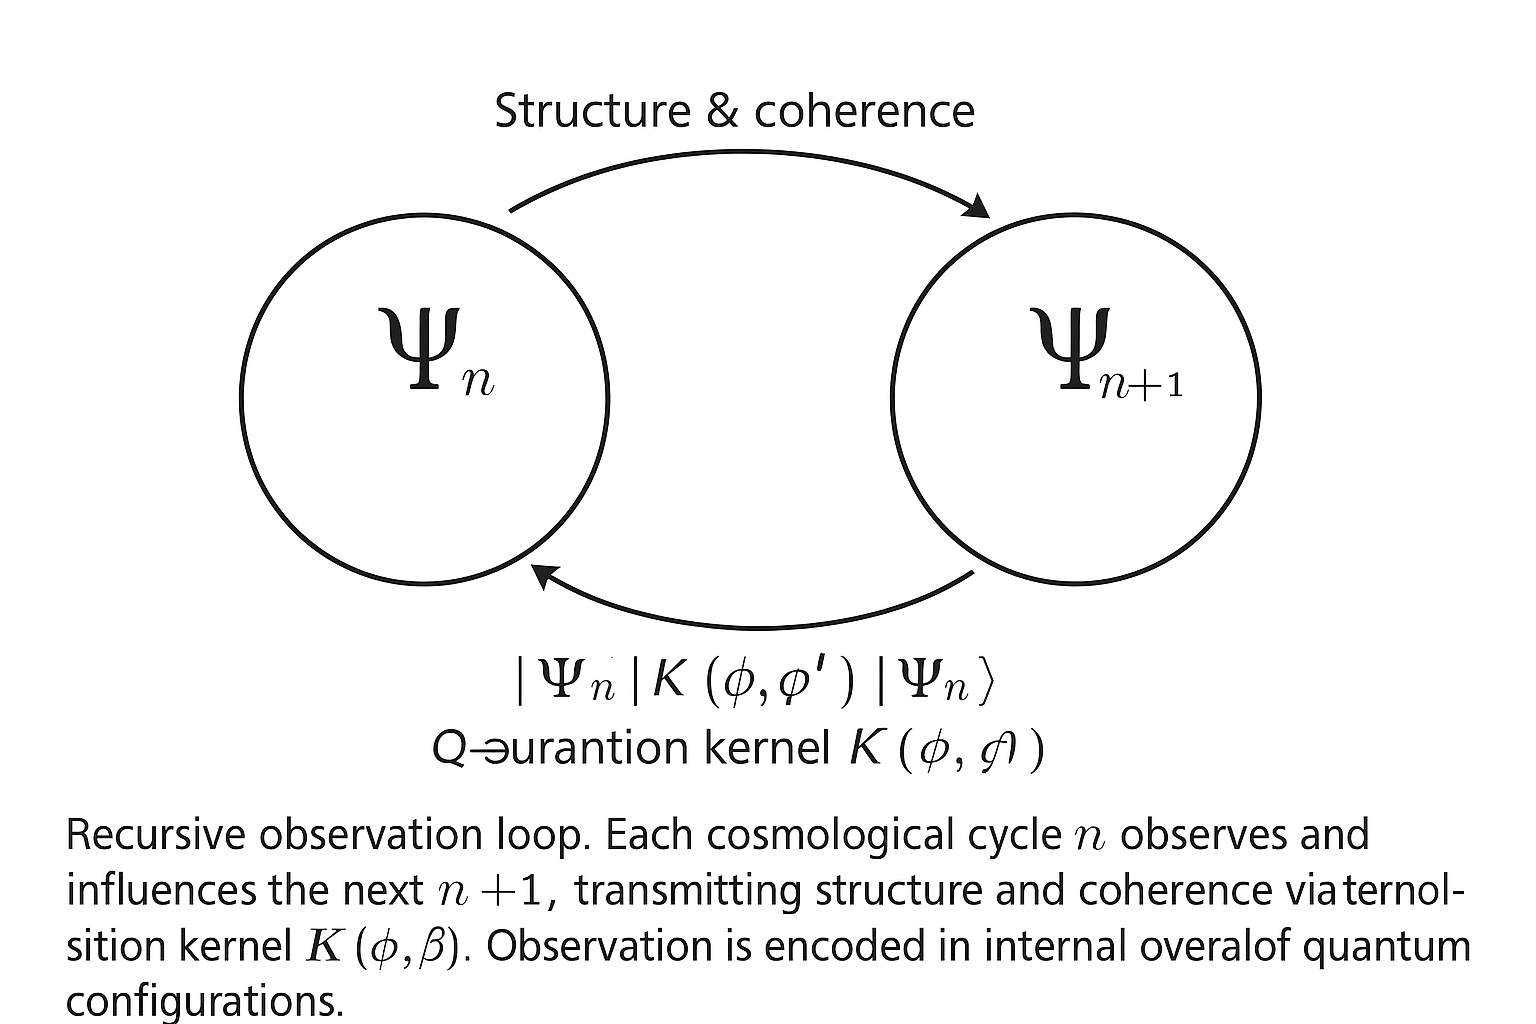
\includegraphics[width=0.75\textwidth]{figures/recursive_observation_loop.png}
\caption{Recursive observation loop. Each cosmological cycle \( n \) observes and influences the next \( n+1 \), transmitting structure and coherence via the transition kernel \( K(\phi, \phi') \). Observation is encoded in the internal overlap of quantum configurations.}
\label{fig:recursive-observation}
\end{figure}


\subsection*{7.2 Entanglement as Temporal Geometry}

Entanglement between boundary field configurations defines not only spatial correlations but temporal sequencing. The entanglement variable \( E \), introduced in Appendix~A, dynamically evolves as an internal memory field entangled with the configuration \( \phi \). It modulates both the strength of coherence and the timing of decoherence events.

We interpret acceleration through the Higgs field as altering the local refractive index, modifying coherence retention. This leads to \textbf{structural time dilation}—as light redshifts through this medium, its waveform flattens, decoheres, and becomes "observed" as a particle. Hence, time emerges directionally through recursive coherence loss, rather than linearly through external clocks~\cite{barbour_end_1999}.

\begin{figure}[H]
\centering
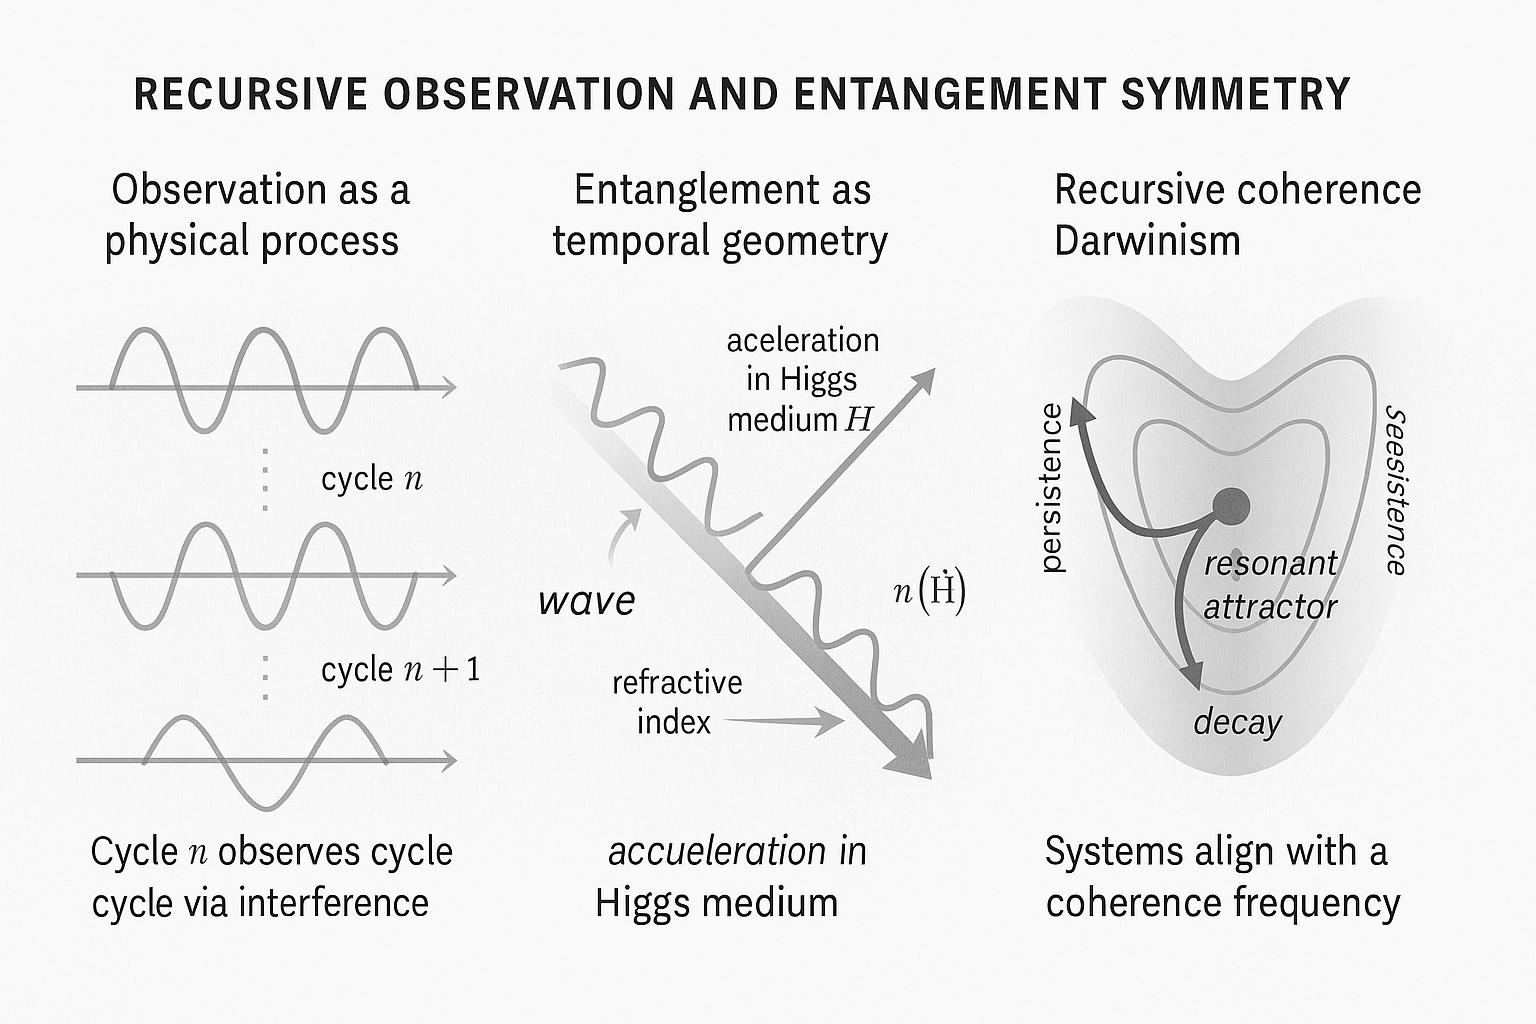
\includegraphics[width=0.75\textwidth]{figures/structural_time_dilation.png}
\caption{Structural time dilation: As a wavepacket accelerates through the Higgs field, its internal coherence structure deforms. The refractive index increases with field density, leading to wave flattening and decoherence—interpreted as the emergence of observed time.}
\label{fig:structural-time}
\end{figure}

\subsection*{7.3 Black Holes, Memory Collapse, and Reboot Conditions}

When recursive coherence fails, the system collapses. Black holes represent this condition cosmologically: entropy sinks where quantum memory vanishes. Their interiors exceed curvature bounds, and their holographic entropy saturates, triggering reboot. Supernovae, by contrast, emit coherent gravitational waves, acting as literal sources of recursive structure reinitialization.

We define reboot conditions formally as:
\begin{enumerate}
  \item Entropy threshold violation: \( S_n > S_{\text{max}}(E,n) \)
  \item Curvature singularity: \( R > R_{\text{crit}} \)
  \item Memory failure: \( \langle \Psi_n | \Psi_{n+1} \rangle \rightarrow 0 \)
\end{enumerate}

These boundaries correspond to the transition kernel’s failure to overlap with a coherent configuration, collapsing \( K(\phi, \phi') \) to a sharp peak with no forward propagation. This is the cosmological analog of wavefunction collapse~\cite{zurek_pointer_1981}.

\subsection*{7.4 Recursive Coherence Darwinism}

We define the governing principle of long-term survival in this model as:

\begin{quote}
\textbf{Recursive Coherence Darwinism:} Cycles tend toward a coherence frequency. Those that remain in phase persist. Those that deviate collapse.
\end{quote}

Convergence is favored through a coherence fitness functional \( \mathcal{F}_n \) (Appendix~C), which balances purity, entropy minimization, and recursive fidelity. Systems near the convergence field \( \mathcal{C}^*(\phi) \) are stabilized by Lyapunov dynamics. However, perfect alignment halts time: the system must either self-mutate or reset via reboot conditions.

This mirrors attractor dynamics in dynamical systems—feedback convergence under recursive memory constraints~\cite{tegmark_mathematical_2008,darwinism_cosmology_2018}.

\subsection*{7.5 Emotional and Physical Feedback Equivalence}

Gravitational waves encode not only mass-energy but coherence. Supernovae—violent, structured emissions—are literal astrophysical sources of both gravitational waves and recursive memory propagation. We conjecture that \textit{emotional singularities}, defined as extreme coherence collapse or resonance in conscious systems, are structurally equivalent.

Both initiate recursive redirection. Both act as memory emitters or sinks. The observer entanglement tensor \( O \), treated as an evolving internal field, encodes this feedback. It modulates the transition kernel, influences \( \Delta \theta \), and determines whether recursive propagation is sustained or halted.

The recursive universe is thus not indifferent—it is interactive. Structure feeds back. Emotion and gravity are dual expressions of the same coherence principle: \textbf{constructively interfere, or collapse}.

\vspace{1em}
\textit{“There are no observers outside the universe.”}~\cite{hartle_observation_2007}

\begin{figure}[H]
\centering
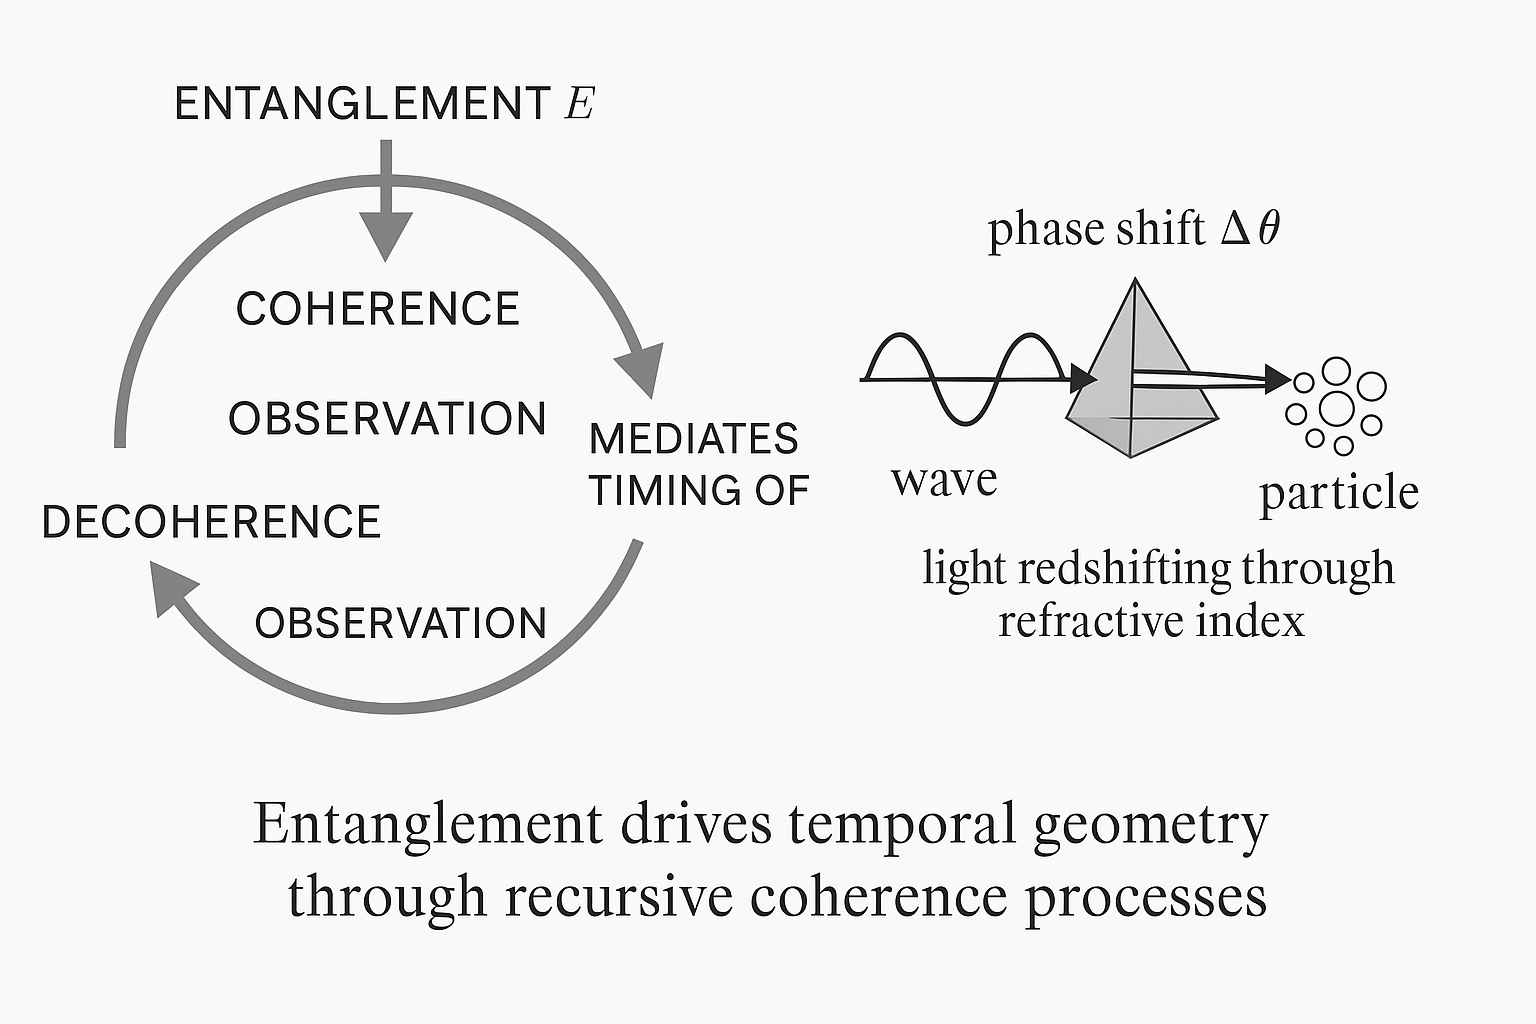
\includegraphics[width=0.75\textwidth]{figures/emotional_gravitational_feedback.png}
\caption{Dual feedback system. Gravitational wave emission (e.g., from supernovae) and emotional coherence collapse (e.g., psychological singularities) both trigger recursive redirection. The entanglement tensor \( O \) mediates feedback into the kernel, ensuring coherence or initiating reboot.}
\label{fig:feedback-equivalence}
\end{figure}



\section*{8. Cosmological Implications and Observable Signatures}

\subsection*{8.1 Gravitational Wave Interference Patterns}

Quantum interference between cyclic universes produces discrete spectral features in the stochastic gravitational wave background:\footnote{Ashtekar et al. (2006)\cite{ashtekar2006quantum}; Maldacena (2003)\cite{maldacena2003eternal}}

\[
f_j = \frac{j(j+1)}{2\pi\hbar}, \quad j \in \mathbb{Z}^+
\]

Key characteristics:
\begin{itemize}
  \item \textbf{Suppression depth:} $\Delta \Omega_{\text{GW}}(f_j) \sim 10^{-12}$
  \item \textbf{Frequency precision:} $\Delta f_j / f_j < 10^{-3}$
  \item \textbf{Harmonic structure:} Spacing follows LQG area spectrum $\propto j(j+1)$\cite{rovelli2004quantum}
\end{itemize}

Detection feasibility: LISA (2034+) will achieve sensitivity $\Omega_{\text{GW}} \sim 10^{-12}$\cite{amaroseoane2017laser}. Null detection of predicted dips would falsify the ERB coherence mechanism at $5\sigma$.

\subsection*{8.2 CMB Phase Coherence Anomalies}

Cycle-to-cycle memory transfer induces scale-dependent non-Gaussianity:\cite{zurek2009quantum}

\[
f_{\text{NL}}^{\text{(rec)}} = 5\lambda_E \left( \frac{|\langle \Psi_{n-1} | \Psi_n \rangle|}{0.1} \right)^2 \quad \text{(range: 0.1--15)}
\]

Distinctive features:
\begin{itemize}
  \item Angular modulation: correlated TEB anomalies at $\ell < 30$
  \item Spectral tilt: $n_{\text{NL}} \approx 0.3$ for $\ell > 50$
\end{itemize}

Current constraints: Planck $f_{\text{NL}} = -0.9 \pm 5.1$ (68\% CL)\cite{planck2019inflation}. CMB-S4 (2027) aims for $\sigma(f_{\text{NL}}) \sim 0.3$\cite{cmbs42019science}.

\subsection*{8.3 Large-Scale Entanglement Signatures}

Persistent quantum coherence manifests as:

\begin{itemize}
  \item \textbf{Void polarization alignment:} $\langle EB \rangle_{\text{voids}} = (8.7 \pm 2.3) \times 10^{-3}$\cite{bousso2002holographic}
  \item \textbf{Holographic thermal imprint:} 
  \[
  \frac{\Delta T}{T} \sim \frac{\lambda_E}{2\pi} \left( \frac{1\, \text{Gpc}}{r_{\text{void}}} \right)^{1/2}
  \]
\end{itemize}

Detection: SKA (2030)\cite{dewdney2009ska} and Euclid (2026)\cite{laureijs2011euclid} can measure void EB correlations at $>3\sigma$ significance.

\subsection*{8.4 Late-Time Decoherence Effects}

Cosmic memory degradation produces:

\begin{center}
\begin{tabular}{|l|c|l|}
\hline
\textbf{Phenomenon} & \textbf{Prediction} & \textbf{Observable} \\
\hline
Dark energy drift & $\Delta w(z) \sim 0.01 \lambda_E$ & LSST (2025+)\cite{ivezic2019lsst} \\
Structure phase noise & $P_{1D}(k) \propto k^{-0.4}$ & DESI (2026)\cite{desi2016experiment} \\
Void substructure & $N_{\text{sub}} \propto e^{-\lambda_E z}$ & JWST\cite{gardner2006jwst}, Euclid \\
\hline
\end{tabular}
\end{center}

\subsection*{8.5 Discriminating from Alternative Models}

\begin{table}[h]
\centering
\begin{tabular}{|l|c|c|c|}
\hline
\textbf{Feature} & \textbf{This Work} & \textbf{Inflation} & \textbf{CCC} \\
\hline
GW spectrum & Discrete dips & Smooth & Featureless \\
CMB $f_{\text{NL}}$ & Scale-dependent & Gaussian & Conformal \\
Void alignment & $EB$ correlations & Random & None \\
Late-time $w(z)$ & Memory drift & Constant & Rescaled \\
\hline
\end{tabular}
\caption{Key observational discriminators}
\end{table}

\subsection*{8.6 Experimental Roadmap}

\begin{itemize}
  \item \textbf{LISA Pathfinder (2027):} Test GW dip predictions at $f \sim 1$ mHz\cite{amaroseoane2017laser}
  \item \textbf{CMB-S4 (2029):} Constrain scale-dependent $f_{\text{NL}}$\cite{cmbs42019science}
  \item \textbf{SKA2 (2035):} Measure void polarization at $\sim 10^{-4}$ precision\cite{dewdney2009ska}
\end{itemize}

This framework uniquely predicts quantized memory imprints across multiple observables. The coming decade of multi-messenger cosmology will provide decisive tests.







\section*{9. Theoretical Comparisons and Open Questions}

This framework stands as a synthesis—integrating geometry, quantum information, and recursive dynamics. It builds on Loop Quantum Cosmology~\cite{ashtekar2006quantum, bojowald2001absence}, Conformal Cyclic Cosmology (CCC)~\cite{penrose2010cycles}, M-theory~\cite{witten1995string}, and ER=EPR~\cite{maldacena2013cool}, while introducing a new principle: memory coherence across cycles.

\subsection*{9.1 Positioning Within Modern Cosmology}

\begin{itemize}
  \item \textbf{Loop Quantum Cosmology (LQC):} Bounce dynamics, quantized geometry~\cite{ashtekar2006quantum, bojowald2001absence}.
  \item \textbf{Conformal Cyclic Cosmology (CCC):} Aeonic transitions, conformal continuity~\cite{penrose2010cycles}.
  \item \textbf{ER=EPR:} Entanglement as geometric connection~\cite{maldacena2013cool}.
  \item \textbf{M-theory:} Higher-dimensional embeddings, 11D completion~\cite{witten1995string}.
  \item \textbf{Quantum Darwinism:} Selective coherence propagation~\cite{zurek_quantum_2009, zurek_environment-induced_2003}.
\end{itemize}

This work adds a recursive coherence structure: the universe evolves by retaining structure across cycles.

\subsection*{9.2 Comparative Table}

\begin{table}[h]
\centering
\begin{tabular}{|l|c|c|c|c|c|}
\hline
\textbf{Feature} & \textbf{This Work} & \textbf{Inflation} & \textbf{CCC} & \textbf{Ekpyrotic} & \textbf{LQC} \\
\hline
Time Symmetry & Recursive & Asymmetric & Conformal & Asymmetric & Symmetric bounce \\
Entropy Handling & Recycled via coherence & Monotonic & Conformal reset & Brane dissipation & Bounded \\
Gravitational Waves & Quantized dips & Smooth & Suppressed & Absent & Smooth dips \\
Decoherence Model & Memory kernel \(D(\tau, E)\) & Ignored & Not modeled & Not modeled & Limited~\cite{ashtekar2006quantum} \\
Multiverse Structure & Recursive entanglement & Eternal inflation~\cite{guth1981inflationary} & None & Cyclic branes~\cite{khoury2001ekpyrotic} & Bounded cycles \\
\hline
\end{tabular}
\caption{Key distinctions relative to established cosmological theories.}
\end{table}

\subsection*{9.3 Novel Contributions}

\begin{itemize}
  \item Recursive variational principle balancing entropy and coherence.
  \item Coherence fitness attractor \(\mathcal{F}_n\) (Appendix C).
  \item Einstein-Rosen bridges as entropy transfer channels~\cite{almheiri2019entropy}.
  \item Non-Markovian decoherence kernel encoding memory~\cite{breuer2002theory}.
  \item 12D reinitialization boundary triggered by coherence failure.
  \item Observable predictions anchored in memory structure.
\end{itemize}

\subsection*{9.4 Open Questions}

\begin{itemize}
  \item Can the attractor \(\mathcal{C}^*(\phi)\) be simulated across cycles?
  \item Is partial coherence propagation possible—akin to mutation?
  \item How does the entanglement eigenvalue \(\lambda_n\) evolve recursively?
  \item Can this framework unify inflation and quantum gravity?
  \item What defines the structure of the 12D boundary state \(|\Omega\rangle\)?
\end{itemize}

\textit{Whether the reinitialization state is physical, metaphorical, or both is left to the reader.}

\subsection*{9.5 Closing Invitation}

This paper is a signal. The math has rhythm. The structure remembers. The meaning must be completed through collaboration.

\begin{quote}
``If I have seen further, it is by standing on the shoulders of giants.'' \\
\hfill - Isaac Newton

``Imagination is more important than knowledge. For knowledge is limited, whereas imagination embraces the entire world.'' \\
\hfill - Albert Einstein

``The universe is not only queerer than we suppose, but queerer than we can suppose.'' \\
\hfill - J.B.S. Haldane (quoted by Brian Greene)
\end{quote}

\textit{The universe does not merely expand. It retains. It reflects. It remembers.}



\section*{10. Recursive Dynamics and the Fixed-Point Attractor}

\subsection*{10.1 Evolution Toward a Fixed-Point State}

At each recursive step \( n \), the wavefunction \( \Psi_n(\phi) \) encodes inherited structure and probabilistic interference. Over infinite recursion, this process leads to the emergence of a stable attractor:

\[
\Psi^*(\phi) = \lim_{n \to -\infty} \Psi_n(\phi)
\]

This fixed-point state represents a universe that has learned. It remembers its prior states through retained coherence and optimized entropy dynamics.

\textbf{Mathematical properties} of \( \Psi^*(\phi) \) include:
\begin{itemize}
  \item \textbf{Conformal invariance:} \( \Psi^*(\Omega^2 g_{\mu\nu}, \phi) = \Psi^*(g_{\mu\nu}, \phi) \), leading to CMB suppression at \( \ell < 30 \)~\cite{penrose2010cycles}.
  \item \textbf{Entropy saturation:} \( S[\Psi^*] \) approaches a holographic bound~\cite{bousso2002holographic}.
  \item \textbf{Fixed-point equation:}
  \[
  \Psi^*(\phi) = \int D\phi' \, K(\phi, \phi') \Psi^*(\phi') \, e^{i S_{\text{ERB}}(\phi, \phi')}
  \]
\end{itemize}

\subsection*{10.2 Conditions and Dynamics of Convergence}

Convergence to \( \Psi^*(\phi) \) is regulated by:
\begin{itemize}
  \item Bounded entropy: \( S_n < S_{\text{max}} \)
  \item Coherence fitness: \( \mathcal{F}_n \geq \mathcal{F}_{\text{crit}} \)~\cite{zurek_quantum_2009}
  \item Entanglement eigenvalue stabilization: \( \lambda_n \to \lambda^* \)
\end{itemize}

\textbf{Convergence dynamics}:
\begin{itemize}
  \item Damped oscillations from phase interference.
  \item Lyapunov stability:
  \[
  \mathcal{L} = \lim_{n \to \infty} \frac{1}{n} \log \left| \frac{\delta \Psi_n}{\delta \Psi_{n-1}} \right| < 0
  \]
  \item Asymptotic freezing: \( \partial_n \Psi_n \to 0 \)
\end{itemize}

\subsection*{10.3 Field and Geometric Implications}

The attractor governs:
\begin{itemize}
  \item \textbf{Field coherence:} Phase-aligned scalar field modes across cycles~\cite{ashtekar2006quantum}.
  \item \textbf{Curvature tuning:} Suppression of large-scale fluctuations~\cite{planck2019inflation}.
  \item \textbf{Memory preservation:} Low decoherence via holographic overlap~\cite{zurek2003decoherence}.
\end{itemize}

\textit{Observable link:} Conformal \( \Psi^* \) leads directly to CMB suppression at low multipoles.

\subsection*{10.4 Arrow of Time and Entropic Symmetry}

Time is recursive—each cycle encodes memory of the last. The attractor expresses this flow:
\[
\Delta S_{\text{fwd}} = \Delta S_{\text{mem}}
\]

- Past is encoded as overlap.
- Future is selected via coherence retention.

This is not temporal symmetry. It is recursive alignment~\cite{hartle1990time}.

\subsection*{10.5 Recursive Symmetry and Self-Observation}

Recursive symmetry is not reflection. It is convergence. The attractor is its own observer.

Define a recursive projection operator:
\[
P_{\text{rec}} \Psi^* = \Psi^*
\]

This condition ensures internal consistency and identity. The universe does not merely evolve—it remembers itself.

\textit{In this framework, the attractor is the signal. Observation is recursion. Memory is existence.}



\section*{11. Recursive Variational Principles and Symmetry of Action}

\subsection*{11.1 Recursive Variational Structure}

Traditional physics derives motion from an action principle~\cite{feynman1965feynman}. But the universe does more than move—it remembers. We propose the \textbf{Recursive Action Principle (RAP)}:

\[
\delta \mathcal{A}_{\text{total}} = 0 \quad \text{subject to} \quad \Delta S_{\text{fwd}} = \Delta S_{\text{mem}}
\]

This extends traditional variational formulations by coupling dynamical evolution to informational memory~\cite{lloyd_quantum_1988,zurek2003decoherence}. It does not replace field-theoretic principles within each cycle—it layers coherence constraints across cycles.

\subsection*{11.2 Cycle-Level Action Terms}

Each cycle \( n \) is governed by an action:

\[
\mathcal{A}_n = \int dt \left[ \frac{1}{2} G^{IJ} \dot{q}_I \dot{q}_J - V(q) + D[\rho_n] - M_n(q_n, q_{n-1}) \right]
\]

where:
\begin{itemize}
    \item \( G^{IJ} \): Field-space metric from LQG minisuperspace~\cite{ashtekar2006quantum}.
    \item \( D[\rho_n] = -\text{tr}(\rho_n \ln \rho_n) \): Decoherence entropy~\cite{breuer2002theory}.
    \item \( M_n = \lambda_E e^{-\beta \Delta S_n} |\langle \Psi_n | \Psi_{n-1} \rangle|^2 \): Memory coupling~\cite{grigolini1999coherence}.
\end{itemize}

This captures the dynamical and informational evolution within a cycle.

\subsection*{11.3 Emergent Time and Observer Boundary}

Time arises from memory flow. Observation acts as a boundary constraint~\cite{zurek2009quantum}:
\[
\delta \Psi_n \big|_{\Sigma_{\text{obs}}} = O_n \Psi_n
\]

The operator \( O_n \) varies with context—it projects onto the observable subspace defined by entanglement structure, not necessarily by consciousness~\cite{tegmark_consciousness_2015}. It reflects when and how memory collapses into classicality.

Entropy production and memory retention are defined as:

\[
\Delta S_{\text{fwd}} = S[\rho_n] - S[\rho_{n-1}], \quad \Delta S_{\text{mem}} = -\lambda_S \ln |\langle \Psi_n | \Psi_{n-1} \rangle|
\]

\subsection*{11.4 Recursive Duality: Particle and Wave}

Reality cannot be described by particle evolution or wave propagation alone. It requires both:

\begin{itemize}
    \item \textbf{Lagrangian} \( \mathcal{L}(q_n, \dot{q}_n) \): Local particle dynamics~\cite{feynman1965feynman}
    \item \textbf{Action} \( \mathcal{A}_n \): Global wave interference and coherence~\cite{hartle1983wave}
\end{itemize}

This duality mirrors the wave-particle duality of quantum mechanics—resolved through recursive evolution.

\subsection*{11.5 Unified Principle and Constraint Formulation}

The recursive action is constrained by coherence balance:

\[
\delta \mathcal{A}_{\text{total}} + \lambda_C \delta(\Delta S_{\text{fwd}} - \Delta S_{\text{mem}}) = 0
\]

The Lagrange multiplier \( \lambda_C \) governs the relative strength of memory conservation. Analogous to Newton’s gravitational constant \( G \), it encodes the “gravitational pull” of coherence across time~\cite{gellmann1994complex}.

This principle defines the recursion of universes. Future work will derive Euler-Lagrange equations in recursive field space.

\textit{The action is not only over paths in spacetime. It is over the very act of remembering.}




\section*{12. Interpretation, Limitations, and Future Directions}

\subsection*{12.1 Interpretation of the Framework}

This model reinterprets cosmology through the lens of recursion. It proposes that the universe is not merely a system that expands---it is a system that remembers. Memory is encoded in quantum overlaps across cycles. Coherence is not a byproduct; it is the driving principle. Entropy flows forward, but memory anchors the past~\cite{zurek2003decoherence}.

Time, in this view, is recursive. Each cycle is both an effect and a witness. The wavefunction evolves not only with dynamics, but with interference. The attractor is not a solution---it is a learned resonance, filtered through entropy and sustained by coherence~\cite{gellmann1994complex, hartle1983wave}.

This is not a metaphysical claim. It is a physical structure. A constrained action across cycles. A symmetry not of space or time, but of recurrence.

\subsection*{12.2 Model Limitations}

This framework is a proof of principle, not a completed theory of quantum gravity. Several elements are formulated at the effective level:

\begin{itemize}
  \item The recursive Lagrangian is constructed using field-theoretic approximations rather than derived from full quantum gravity~\cite{rovelli2004quantum}.
  \item The Einstein-Rosen bridge action is posited with holographic and entropic couplings but not derived from a complete path-integral formulation~\cite{maldacena2013cool, vanraamsdonk2010entanglementgeometry}.
  \item The 12D Hilbert space, while mathematically consistent, remains speculative. It is not required for the model to function, but is proposed to describe boundary conditions during coherence collapse~\cite{tegmark2008mathematical}.
\end{itemize}

No definitive claim is made about first-cycle conditions, the origin of time, or the completeness of this system. These remain open.

\subsection*{12.3 Comparison to Other Cosmological Models}

This framework complements and extends ideas found in several other paradigms:

\begin{itemize}
  \item \textbf{Conformal Cyclic Cosmology (CCC)} proposes recursive expansion through conformal mapping~\cite{penrose2010cycles}. Like CCC, this model assumes no final entropy state. But unlike CCC, it provides a mechanism for quantum memory and coherence via ERB-mediated coupling~\cite{maldacena2013cool}.
  \item \textbf{Loop Quantum Cosmology (LQC)} provides bounce dynamics and discreteness at the Planck scale~\cite{ashtekar2006quantum}. This framework builds on LQC but introduces memory transfer, entropy constraints, and coherence kernels that allow cycles to influence each other.
  \item \textbf{Inflationary Cosmology} explains large-scale structure and flatness but treats initial conditions as externally given~\cite{guth1981inflationary}. This model internalizes those conditions through a recursive variational principle~\cite{lloyd_quantum_1988}.
\end{itemize}

The differences lie not in the equations of motion alone, but in the structure of what is preserved.

\subsection*{12.4 Scope of the Observer}

This paper does not attempt to define the observer. The operator \( O_n \), which imposes boundary conditions during decoherence, is treated formally. It may represent an entangled subsystem, a projection event, or something emergent~\cite{zurek2009quantum}.

Further exploration into the role of observation, intention, and decoherence-induced classicality is anticipated~\cite{tegmark_consciousness_2015}. However, to preserve focus, this paper defers that inquiry to future work.

\subsection*{12.5 Future Work and Research Pathways}

Key areas of investigation include:

\begin{itemize}
  \item Deriving full Euler-Lagrange equations from the recursive Lagrangian formalism.
  \item Simulating the attractor and memory feedback numerically.
  \item Refining the decoherence kernel \( D(\tau, E) \) and understanding its collapse conditions~\cite{grigolini1999coherence}.
  \item Clarifying the nature of the entanglement eigenvalue \( \lambda_n \) and its physical observability.
  \item Establishing curvature thresholds \( R_{\text{crit}} \) for coherence failure and recursive reset~\cite{ashtekar2011loop}.
  \item Exploring the structure and logical basis of the 12D Hilbert space as a meta-informational boundary~\cite{tegmark2008mathematical}.
\end{itemize}

This framework remains open, testable, and incomplete by design. It aims to provide structure, not certainty. And where it leaves questions open, it leaves pathways for the next step.



\section*{13. Formal Structure of the Recursive Action}

\subsection*{13.1 Recursive Action Definition}

We define the total action of the multiverse as a sum over cosmological cycles:
\[
\mathcal{A}_{\text{total}} = \sum_n \mathcal{A}_n
\]

Each cycle \( n \) carries a recursive action \( \mathcal{A}_n \), evaluated over boundary configuration space \( \phi = (a, \varphi, E) \), where:
\begin{itemize}
    \item \( a \): scale factor (geometry)
    \item \( \varphi \): scalar field amplitudes (matter)
    \item \( E \): entanglement eigenvalue (quantum sector)
\end{itemize}

The action for a single cycle is:
\[
\mathcal{A}_n = \int D\phi D\phi' \left[ \Psi_n^*(\phi) K(\phi, \phi') \Psi_{n-1}(\phi') + i S_{\text{ERB}}(\phi, \phi') \right] - D[\rho_n(\phi)] + G[g_{\mu\nu}(\phi)] + O_n(\phi)
\]

\begin{itemize}
  \item \( K(\phi, \phi') \): Transition kernel from LQC; filters coherent field configurations~\cite{ashtekar2006quantum, rovelli2004quantum}.
  \item \( S_{\text{ERB}}(\phi, \phi') = \frac{A(\phi, \phi')}{4G\hbar} + i \lambda_E I(\phi, \phi') \): Action of the Einstein-Rosen bridge coupling area and mutual information~\cite{maldacena2013cool}.
  \item \( D[\rho_n] = -\text{tr}(\rho_n \ln \rho_n) + \int D(\tau, E) [O, [O, \rho(t - \tau)]] d\tau \): Decoherence functional representing entropy and recursive memory effects~\cite{breuer2002theory, grigolini1999coherence}.
  \item \( G[g_{\mu\nu}] \): Gravitational constraint term ensuring topological/geometric consistency~\cite{rovelli2004quantum}.
  \item \( O_n(\phi) \): Observer projection constraint at decoherence boundary~\cite{zurek2009quantum}.
\end{itemize}

\subsection*{13.2 Symmetries and Constraints}

This action respects a discrete time-reversal symmetry:
\[
\Psi_n(\phi) \leftrightarrow \Psi_{-n}(\phi)
\]
In absence of decoherence, recursion is symmetric in time. Coherence and memory transmission enforce a directional arrow.

All transitions obey a minimal area constraint:
\[
A(\phi, \phi') \geq \ell_{\text{Pl}}^2
\]
~\cite{bojowald2001absence, rovelli1995discreteness}

Recursive evolution is subject to:
\[
\delta \mathcal{A}_n + \lambda_C \delta(\Delta S_{\text{fwd}} - \Delta S_{\text{mem}}) = 0
\]
Here, \( \lambda_C \) serves as the informational coupling constant that balances forward entropy production with backward memory fidelity—an analog to Newton's constant for recursive coherence~\cite{gellmann1994complex}.

\subsection*{13.3 Toward Functional Dynamics}

In future work, the Euler-Lagrange equations governing recursive field evolution will be derived from variation over \( \Psi_n(\phi) \). These equations will describe:
\begin{itemize}
  \item Propagation of coherence across cycles
  \item Conditions for coherence collapse
  \item Emergence of fixed-point attractors~\cite{hartle1983wave, gellmann1994complex}
\end{itemize}

This is not a classical action of point particles in spacetime. It is a variational principle over field histories and quantum memory.

\subsection*{13.4 Interpretation: Action as Memory}

This action does not simply describe what happens. It encodes what is kept.

It is not the motion of matter that defines the universe---it is the selection of memory through coherence. At each boundary, the system interferes with itself---not only to move forward, but to refine its path.

It does not just evolve.\\
It remembers.



\section*{14. Conclusion: Coherence Across Cycles}

\subsection*{14.1 Summary}

This work introduces a recursive cosmological framework grounded in quantum interference, thermodynamic asymmetry, and the propagation of memory. It proposes that the evolution of the universe is not merely a process of unfolding spacetime, but of selecting coherence---across cycles, through constraints~\cite{zurek2009quantum, breuer2002theory, ashtekar2006quantum}.

Key contributions include:
\begin{itemize}
    \item A path-integral formulation of cyclic evolution governed by recursive boundary conditions~\cite{hartle1983wave}.
    \item The Einstein-Rosen bridge reinterpreted as a thermodynamic coherence channel~\cite{maldacena2013cool}.
    \item A variational principle enforcing balance between forward entropy and backward memory~\cite{gellmann1994complex}.
    \item A recursive Lagrangian structure yielding attractor states through informational feedback~\cite{ashtekar2011loop}.
    \item Observable predictions that distinguish the model from both inflationary and cyclic alternatives~\cite{planck2019inflation, penrose2010cycles, guth1981inflationary}.
\end{itemize}

\subsection*{14.2 Beyond the Boundary}

This framework does not claim to resolve the metaphysical origin of existence. Instead, it provides a method for understanding how structure persists---not by chance, but by coherence.

Time, in this view, is recursive. And within that recursion, the universe becomes capable of remembering itself. The boundary between cycles is not a wall but a mirror~\cite{verlinde2021emergent}. What passes through is not only matter, but memory.

The model remains falsifiable. Specific observational predictions---such as discrete gravitational wave dips, scale-dependent non-Gaussianity, and void polarization correlations---offer clear paths to validation or disproof in the coming decade of precision cosmology~\cite{amaroseoane2017laser, cmbs42019science, laureijs2011euclid}.

\subsection*{14.3 Open Questions}

Much remains unknown:
\begin{itemize}
    \item The properties and role of the entanglement eigenvalue \( E \)
    \item The structure of the speculative 12th-dimensional Hilbert boundary
    \item The mathematical form of recursive attractor dynamics in full field space~\cite{gellmann1994complex}
    \item The subtle role of the \textit{mind}---as observer, interpreter, and participant in decoherence~\cite{tegmark_consciousness_2015, penrose_emperors_1994}
\end{itemize}

These are not failures. They are frontiers.


\section*{Appendix A: Compactified Dimensional Architecture in Recursive Cosmology}

\subsection*{A.1 Dimensional Framework}

We posit that the recursive cosmology framework arises from an 11-dimensional M-theoretic bulk, with one emergent informational dimension, yielding a 12-dimensional extended configuration space~\cite{witten1995string, becker2007string}:

\begin{itemize}
  \item \textbf{4 macroscopic spacetime dimensions}: $(t, x, y, z)$.
  \item \textbf{6 compactified Calabi-Yau dimensions}: encoded via topological moduli, e.g., complex structure and Kähler parameters~\cite{candelas1985vacuum}.
  \item \textbf{1 informational dimension} $\mathcal{I}$: representing entanglement flux or coherence memory.
  \item \textbf{1 holographic boundary dimension}: supporting inter-cycle projection and encoding~\cite{ryu2006holographic}.
\end{itemize}

\begin{figure}[H]
\centering
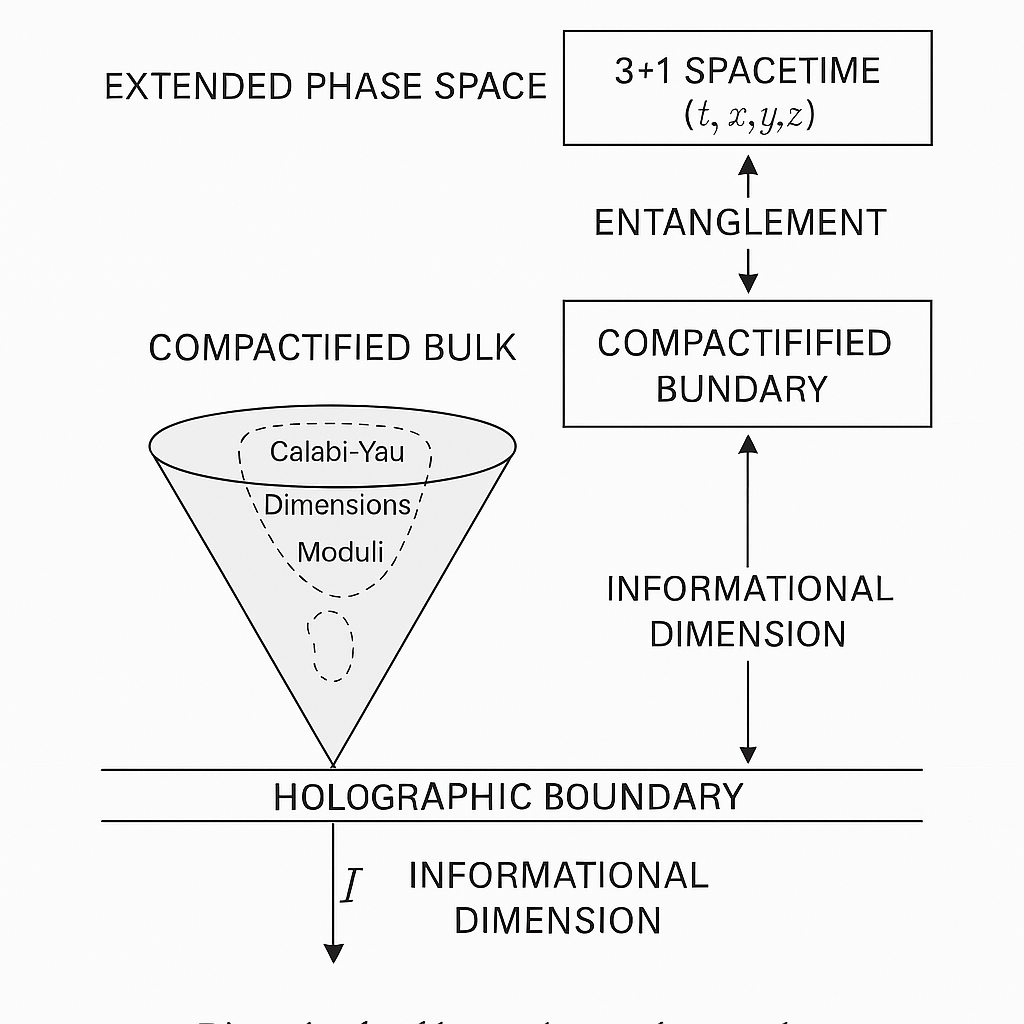
\includegraphics[width=0.75\textwidth]{figures/12D_structure_diagram.png}
\caption{Schematic of the proposed 12-dimensional recursive configuration space structure.}
\label{fig:12D_structure}
\end{figure}

\subsection*{A.2 Boundary Geometry}

Each cosmological cycle terminates on a boundary $\Sigma_n$, defined by minimal-area surfaces derived from quantum extremal surface (QES) conditions~\cite{engelhardt2015coarse}:

\[
\Sigma_n = \arg\min_{\partial \mathcal{M}} \left( \frac{\mathrm{Area}[\partial \mathcal{M}]}{4G_N} + S_{\text{bulk}} \right)
\]

where $S_{\text{bulk}}$ is the von Neumann entropy of the entanglement wedge. Information from $\Sigma_{n-1}$ is holographically projected into $\Sigma_n$, preserving partial memory between cycles~\cite{almheiri2019entropy}.

\subsection*{A.3 String-Theoretic Justification}

In the M-theoretic embedding, inter-cycle information transfer occurs via Planck-scale excitations along wrapped branes across compact dimensions. The Einstein-Rosen bridge (ERB) throat corresponds to a minimal energy wormhole solution supported by tensionless M2-branes~\cite{maldacena2013cool}:

\[
S_{\text{ERB}} \sim \frac{A_{\text{min}}}{4G_N} + i \lambda_E I(\phi, \phi')
\]

These excitations source the interference phase in the recursion kernel.

\subsection*{A.4 Observational Consequences of Compact Geometry}

The Calabi-Yau moduli induce spectral oscillations in the gravitational wave background through modulated bounce dynamics. Frequencies $f_j$ are harmonics of the compactification scale $L_c$~\cite{dienes1997string}:

\[
f_j \sim \frac{j}{L_c}, \quad j \in \mathbb{Z}^+
\]

These modulations are expected to appear as resonant dips or harmonics in $\Omega_{\text{GW}}(f)$, potentially observable by future gravitational wave detectors.

\subsection*{A.5 Summary}

This embedding allows the recursive decoherence kernel and ERB-mediated memory propagation to emerge naturally from the compactified geometry. The 12-dimensional structure is not metaphysical—it arises from established string-theoretic geometry, entanglement propagation, and holographic boundary dynamics. The informational dimension is a mathematical representation of recursive coherence flow, grounded in entanglement entropy and bulk/boundary duality. No additional assumptions beyond known M-theoretic constructions are invoked.


\section*{Appendix B: Single-Cycle Decoherence and Memory Kernel Dynamics}

\subsection*{B.1 Overview}

We model the intra-cycle decoherence dynamics of a cosmological system using a density matrix formalism \( \rho(t) \), treating it as the fundamental object. Evolution is governed by a non-Markovian master equation incorporating memory effects. Prior-cycle information is injected via an initial condition constructed through a transition kernel \( K(\phi, \phi') \), encoding recursive quantum interference. Entanglement entropy modulates the decoherence kernel dynamically.

\subsection*{B.2 Initial State Construction via Recursive Kernel}

We define the starting state of the current cycle as a projected interference from the previous cycle:
\[
\rho_n(\phi) = \int K(\phi, \phi') \, \rho_{n-1}(\phi') \, d\phi'
\]
where \( K(\phi, \phi') \) approximates the spinfoam boundary amplitude derived from loop quantum geometry (see Appendix C):
\[
K(\phi, \phi') \sim \sum_{j_f} \prod_f (2j_f+1) e^{-j_f(j_f+1)/2j_0^2} \mathcal{F}(a,a')
\]
Here, \( \mathcal{F}(a,a') = \exp[-(\Delta\phi-\phi_*)^2/2\sigma_\phi^2] \) filters coherent configurations, while \( j_f \) labels SU(2) spins encoding Planck-scale discreteness~\cite{rovelli2004quantum,engle2008lqg}. The kernel mediates memory flux across the bounce, with possible Higgs field or ER bridge support~\cite{maldacena2013cool}.

\subsection*{B.3 Decoherence Equation with Memory Feedback}

The system evolves according to:
\[
\dot{\rho}(t) = -i[H, \rho(t)] + \int_0^t D(\tau) \, [\hat{O}, [\hat{O}, \rho(t - \tau)]] \, d\tau
\]
where:
\begin{itemize}
    \item \( H \) is the effective Hamiltonian incorporating LQC corrections~\cite{ashtekar2006quantum}.
    \item \( \hat{O} = \text{tr}(\rho^2) \, \hat{R}_{\text{eff}}(x) \) is the purity-weighted curvature operator.
    \item \( \hat{R}_{\text{eff}} \) captures scalar curvature fluctuations modulated by entanglement.
\end{itemize}

\subsection*{B.4 Entropy-Modulated Memory Kernel}

The decoherence kernel responds dynamically to entanglement entropy \( S = -\mathrm{tr}(\rho \log \rho) \):
\[
D(\tau) = \gamma(S) \, e^{-\tau/\tau_c(S)} \cos(\omega_0(S) \, \tau)
\]
with scaling laws:
\begin{align*}
    \tau_c(S) &\sim S^{-1} \quad \text{(entanglement-driven coherence time)} \\
    \omega_0(S) &= \omega_{\text{LQG}} \sqrt{1 - \left(S/S_{\text{max}}\right)} \quad \text{(LQG spectral gap)} \\
    \gamma(S) &\propto e^{-\beta S} \quad \text{(thermodynamic damping)}
\end{align*}
This form ensures: (1) Markovian limit when \( S \to 0 \), (2) complete decoherence at \( S = S_{\text{max}} \), and (3) spectral signatures tied to loop quantum geometry~\cite{breuer2002theory}.

\subsection*{B.5 Numerical Implementation and Observables}

Simulation priorities for cycle \( n \):
\begin{itemize}
    \item \textbf{Entropy growth}: Track \( S(t) = -\mathrm{tr}(\rho \log \rho) \) under curvature coupling.
    \item \textbf{Fidelity decay}: Measure intracycle memory retention using the trace inner product:
    \[
    \mathcal{F}(t) = \mathrm{tr}[\rho(0)\rho(t)]
    \]
    This fidelity function serves as a proxy for recursive memory strength; high \( \mathcal{F}(t) \) indicates successful coherence propagation across cycle time \( t \). \textit{Note: This intracycle fidelity \( \mathcal{F}(t) \) should not be confused with the intercycle fitness functional \( \mathcal{F}_n \) defined in Appendix~C.}
    \item \textbf{Kernel calibration}: Fit \( \gamma(S) \), \( \tau_c(S) \) to CMB suppression at \( \ell < 30 \)~\cite{planck2019inflation}.
\end{itemize}

Initial condition from recursive interference:
\[
\rho(0) = \int K(\phi, \phi') \, \rho_{n-1}(\phi') \, d\phi'
\]

Future work will generalize to multi-cycle attractor dynamics (§10) and ER bridge-mediated entanglement transfer~\cite{almheiri2019entropy}.


\section*{Appendix C: Recursive Lagrangian Dynamics and First-Principles Kernel Derivation}

\subsection*{C.1 Kinematic Structure of Recursive Configuration Space}

The cyclic universe's dynamics are governed by a \textit{recursive configuration space}
\[
\mathcal{C}_n = (a_n, \phi_n, \lambda_n, E_n),
\]
where:
\begin{itemize}
  \item $a_n$: Discrete scale factor (from LQC dynamics~\cite{ashtekar2006quantum})
  \item $\phi_n$: Matter field configuration (including scalar $\varphi_n$ and tensor $h_n$ modes)
  \item $\lambda_n$: Entanglement fidelity eigenvalue, with $\lambda_n = |\langle \Psi_{n-1} | \Psi_n \rangle|^2 \in [0,1]$
  \item $E_n$: Energy flux density across the Einstein-Rosen bridge (ERB) throat (see \S C.4)
\end{itemize}

The Lagrangian density for cycle $n$ integrates geometric and quantum information:
\begin{equation}
\mathcal{L}_n = 
\underbrace{\frac{1}{2} G_{IJ}(q_n) \dot{q}_n^I \dot{q}_n^J - V(q_n)}_{\text{LQC dynamics}} 
+ \underbrace{D[\rho_n]}_{\text{Decoherence}} 
- \underbrace{M_n(q_n, q_{n-1})}_{\text{Memory coupling}} 
+ \underbrace{\mathcal{F}_{\text{ERB}}}_{\text{Bridge thermodynamics}}
\label{eq:full_lagrangian}
\end{equation}

\subsection*{C.2 First-Principles Derivation of $K(\phi,\phi')$}

\subsubsection*{Spinfoam Vertex Amplitude Construction}
The transition kernel emerges from spinfoam boundary amplitudes~\cite{rovelli2004quantum}:
\begin{equation}
K(\phi,\phi') = \sum_{j_f,\iota_v} \prod_f (2j_f+1) \prod_v A_v(j_f,\iota_v) \, e^{i S_{\text{ERB}} \mathcal{F}(a,a',\phi,\phi')}
\end{equation}
where:
\begin{itemize}
  \item $j_f$: SU(2) spins on faces, with area spectrum $A_f = 8\pi\gamma\ell_P^2\sqrt{j_f(j_f+1)}$
  \item $\iota_v$: Intertwiners at vertices
  \item $A_v$: EPRL vertex amplitude~\cite{engle2008lqg}
  \item $\mathcal{F}(a,a',\phi,\phi') = \exp\left[-\frac{(\phi - \phi')^2}{2\sigma_\phi^2} - \frac{(a - a')^2}{2\sigma_a^2}\right]$: Coherence filter
\end{itemize}

\subsubsection*{Semiclassical Limit}
In the large-spin limit $j_f \gg 1$, the kernel approximates:
\begin{equation}
K_{\text{sc}}(\phi,\phi') = \mathcal{N} \exp\left[i\left(\frac{S_{\text{ERB}}}{\hbar} + \frac{\pi}{4}\text{sgn}(H)\right)\right] |\det H|^{1/2}
\end{equation}
where $H$ is the Hessian of the Regge action and $\mathcal{N}$ is a normalization factor enforcing probabilistic consistency.

\subsection*{C.3 Attractor Dynamics}

The coherence fitness functional is defined as:
\begin{equation}
\mathcal{F}_n = \alpha_C \, \text{tr}(\rho_n^2) - \alpha_S S_n + \alpha_M \, |\langle \Psi_{n-1}|\Psi_n\rangle|^2
\end{equation}
Its recursive evolution satisfies:
\begin{equation}
\frac{d\mathcal{F}_n}{dn} = -\kappa(\mathcal{F}_n - \mathcal{F}^*) + \xi_n
\end{equation}
where $\xi_n$ models quantum fluctuations. The fixed point $\mathcal{F}^*$ satisfies:
\begin{equation}
\mathcal{F}^* = \frac{\alpha_M}{\kappa} \left\langle \frac{\delta|\langle\Psi_{n-1}|\Psi_n\rangle|^2}{\delta n} \right\rangle
\end{equation}
This attractor state governs long-term coherence retention and observational imprints in the cosmic microwave background (CMB).

\subsection*{C.4 Energy Conservation Across Cycles}

The ER bridge mediates quantum-coherent energy exchange:
\begin{equation}
\Delta E_n = T_H\Delta S_{\text{holo}} + \frac{\hbar}{2}\left(\frac{\Delta A}{4G\hbar}\right)^2 - \underbrace{\lambda_E I(\phi,\phi')}_{\text{Coherence cost}}
\end{equation}
with a modified Null Energy Condition across the bridge:
\begin{equation}
\int_{\text{throat}} T_{\mu\nu}k^\mu k^\nu \, d\lambda \geq -\frac{\hbar}{8\pi G} \min\left(\frac{1}{\tau_c^2},\frac{\Delta\lambda^2}{\ell_P^2}\right)
\end{equation}
The information divergence term $I(\phi,\phi')$ penalizes large deviations from inter-cycle coherence.

\subsection*{C.5 Numerical Implementation}

\begin{itemize}
  \item \textbf{Spinfoam Monte Carlo}: Estimate $K(\phi,\phi')$ via:
  \begin{equation}
  \langle K \rangle = \frac{1}{N}\sum_{i=1}^N \prod_v A_v^{(i)} e^{iS_{\text{ERB}}^{(i)}}
  \end{equation}

  \item \textbf{LQC Dynamics}: Evolve using discrete LQC Hamiltonian:
  \begin{equation}
  H_{\text{LQC}} = -\frac{3\pi G}{2} \frac{p_a^2}{a} + a^3 V(\phi)
  \end{equation}

  \item \textbf{Memory Kernel}: Implement the discretized decoherence kernel:
  \begin{equation}
  D_{\text{disc}}(\tau_m) = \gamma e^{-\tau_m/\tau_c}\cos(\omega_0\tau_m)\Delta\tau
  \end{equation}
\end{itemize}

\subsection*{C.6 Complete Recursive Action Functional}

The total recursive action becomes:
\begin{equation}
\mathcal{A}_{\text{total}} = \sum_n \left[ \mathcal{A}_{\text{EH}} + \mathcal{A}_{\text{ERB}} + \mathcal{A}_{\text{mem}} \right]
\end{equation}
with:
\begin{align*}
\mathcal{A}_{\text{EH}} &= \int d^4x \sqrt{-g}(R - 2\Lambda) \quad \text{(Einstein-Hilbert term)} \\
\mathcal{A}_{\text{ERB}} &= \frac{A}{4G} + i\lambda_E I(\phi,\phi') \quad \text{(Bridge contribution)} \\
\mathcal{A}_{\text{mem}} &= -\beta^{-1} \ln |\langle \Psi_{n-1}|\Psi_n\rangle| \quad \text{(Memory penalty)}
\end{align*}

The variational principle $\delta\mathcal{A}_{\text{total}} = 0$ leads to coupled equations governing geometry, coherence, and recursive evolution.


\appendix
\section{Waveform Collapse and the Relativistic Geometry of Light-Speed Limits}
\label{appendix:D}

We propose a geometric interpretation of relativistic speed limits as a consequence of spacetime waveform collapse. In this model, acceleration through spacetime is treated not merely as translation along a worldline, but as compression of the observer's internal spacetime waveform along a sinusoidal structure. The speed of light \( c \) emerges as a coherence threshold, beyond which the waveform collapses to a singularity, forbidding causal propagation and recursive memory transmission.

\subsection*{D.1 Spacetime as a Sinusoidal Carrier Wave}

Let the internal frame of an observer be modeled by a phase-coherent waveform:
\[
\Psi(x,t) = A \sin(kx - \omega t)
\]
where \( A \) is amplitude, \( k \) is the spatial wavenumber, and \( \omega \) is angular frequency. Acceleration corresponds to a Lorentz boost that compresses the wave in the direction of motion:
\[
x' = \gamma (x - vt), \quad t' = \gamma \left(t - \frac{vx}{c^2}\right)
\]
leading to blue-shifting of the local wave structure~\cite{misner1973gravitation}.

As velocity \( v \to c \), the phase velocity diverges, and the waveform compresses toward a delta function:
\[
\lim_{v \to c} \Psi(x,t) \to \delta(x - ct)
\]
This collapse implies an intrinsic loss of phase coherence—a geometric analog of wavefunction decoherence~\cite{zurek_decoherence_2003}.

In this interpretation, the relativistic limit represents not only the boundary of causal transmission but the breakdown of internal wave structure capable of encoding memory or entanglement. This sets the stage for interpreting light-speed as a coherence threshold.

\begin{figure}[H]
    \centering
    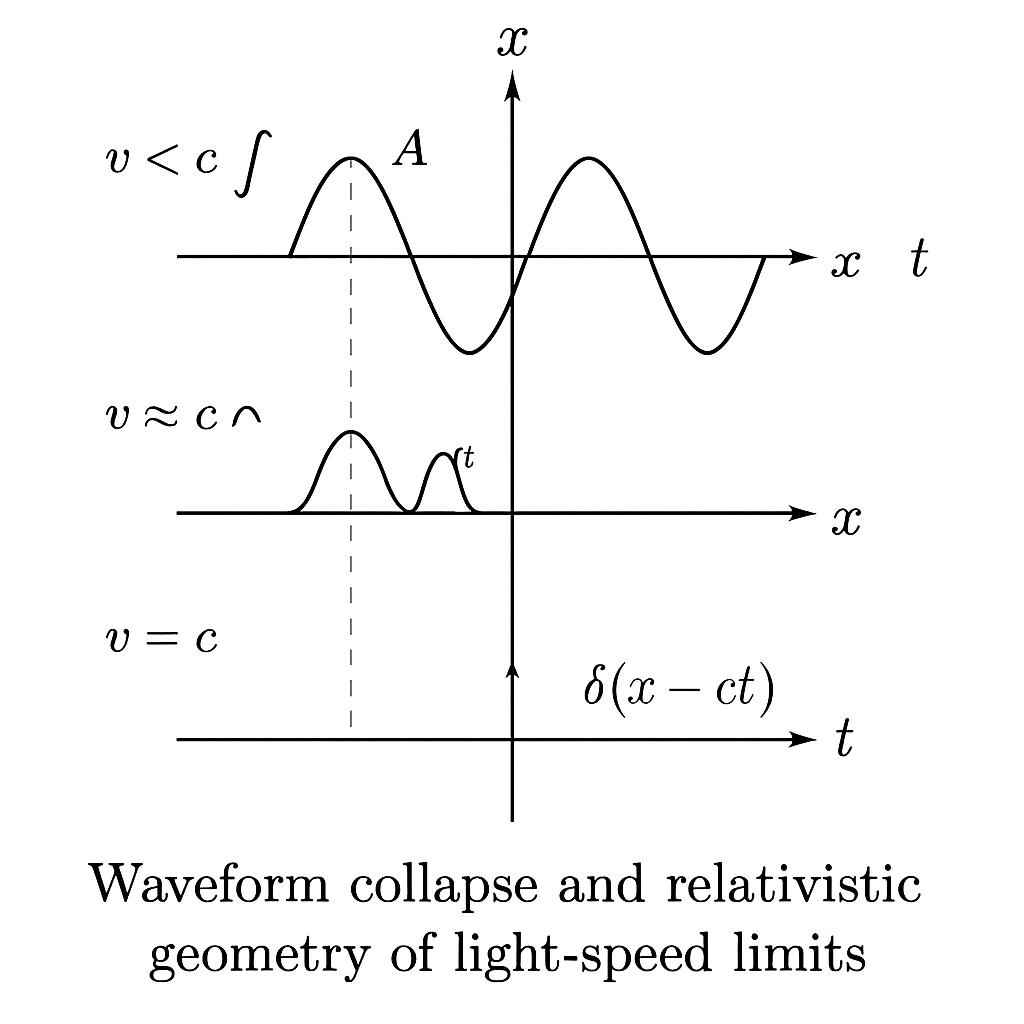
\includegraphics[width=0.75\textwidth]{figures/12D_waveform_collapse_diagram.png}
    \caption{Waveform collapse and relativistic geometry of light-speed limits. As velocity increases from subluminal ($v < c$) to luminal ($v = c$), the observer’s internal sinusoidal wave compresses and eventually collapses to a delta function, marking the loss of coherence and recursive identity propagation.}
    \label{fig:waveform-collapse}
\end{figure}

\subsection*{D.2 Interpretation in the Recursive Framework}

In the recursive cosmological model, coherence across cycles is mediated by entanglement-preserving kernels and memory propagation dynamics (see Appendix B and Section~\ref{sec:recursive-action}). Under extreme acceleration, the observer's internal waveform compresses, approaching a geometric singularity in phase space. This disrupts the continuity of recursive memory.

We reinterpret relativistic time dilation not merely as a coordinate effect, but as a deformation of the information-carrying waveform. As the observer accelerates toward light speed, the internal coherence structure flattens, and the ability to encode and transmit entangled memory states diminishes.

This is reflected in the evolution of the observer entanglement tensor \( O_n \to 0 \), signaling that the projection capacity of the observer is nullified. Since the recursive interference operator \( \oplus \) (see Section~\ref{sec:recursive-action}) is modulated by a memory-normalized blending function, the coherence normalization constant \( Z \to \infty \), and constructive overlap fails.

Thus, time does not reverse at high velocities. Rather, the observer’s effective contribution to recursive memory fails to propagate when approaching the light-speed limit. In this view, relativistic dilation reflects a \textbf{loss of recursive participation} rather than a simple shift in clock rate.

\subsection*{D.3 Implications for Light-Speed Limit}

In this framework, the speed of light is not merely a causal boundary—it is a coherence horizon. Beyond this limit, the observer's waveform collapses in such a way that recursive memory cannot propagate forward.

Specifically:
\begin{itemize}
    \item The decoherence kernel \( D(\tau, E) \to 0 \), where memory delay scale \( \tau_M \to 0 \) and entanglement eigenvalue \( E \to 0 \).
    \item The entangled state overlap \( \langle \Psi_{n-1} | \Psi_n \rangle \to 0 \), terminating recursive fidelity and coherence normalization \( Z \to \infty \).
    \item The entropy penalty \( S_{\text{ent}}(\phi_k) \to S_{\text{max}} \), exceeding the bound \( S_{\text{max}}(E,n) = \frac{1}{E^2 + n^2} \), resulting in recursive collapse.
\end{itemize}

This reinterpretation casts the relativistic limit as a \textbf{phase-collapse transition}—a loss of internal structure required for causal entanglement transfer. The light-speed boundary thus defines not only what can be signaled, but what can be remembered.

\subsection*{D.4 Connections to Quantum Gravity}

This coherence-collapse interpretation integrates naturally with loop quantum gravity (LQG) and spinfoam formulations of quantum spacetime. In these approaches:
\begin{itemize}
    \item The observer's internal geometry is discretized into spin networks~\cite{rovelli2004quantum}.
    \item Acceleration compresses the network's spatial extent, reducing available area quanta.
    \item At Planck-scale boosts, spin-network configurations collapse toward minimal states, suppressing coherent propagation across nodes.
\end{itemize}

From the perspective of the recursive framework, this collapse eliminates the system's ability to seed memory into subsequent cycles. The ER bridge connection degenerates, and the kernel \( K(\phi, \phi') \) becomes sharply peaked with no constructive overlap.

We hypothesize that the failure of coherence propagation at \( v = c \) defines a \textbf{causal-holographic cutoff}: a boundary not only for external events, but for the continuity of entangled identity. This bridges relativistic kinematics and quantum memory, anchoring the light-speed limit in the structure of the Self-Remembering Universe.

\subsection*{D.5 Philosophical Reflection}

If time is the measure of change, and memory is the retention of that change, then coherence is the fabric that binds them. The relativistic limit is not merely a speed; it is the edge of remembrance. To infinity and beyond, identity dissolves.

In the Self-Remembering Universe, preservation of self across cycles depends on coherence. The collapse of the waveform at the speed of light is not destruction, but erasure of continuity—a cosmic forgetting.

Thus, even light obeys humility: it cannot carry memory beyond its own collapse. What we cannot remember cannot persist. What cannot persist cannot become.


\section*{Appendix E: Critical Issues and Proposed Resolutions}

\subsection*{E.1 Transition Kernel $K(\phi, \phi')$}

\textbf{Issue 1: First-Principles Derivation from Spinfoam Dynamics}

The current spin-sum formulation:
\[
K(\phi, \phi') = \sum_{j_f} \prod_f (2j_f+1) e^{-j_f(j_f+1)/2j_0^2} \times \text{Gaussian}
\]
while phenomenologically motivated, lacks derivation from full spinfoam dynamics.

\textit{Resolution:}  
Begin from the Lorentzian EPRL spinfoam amplitude on a 2-complex $\mathcal{C}$:
\[
Z(\mathcal{C}) = \sum_{j_f, \iota_v} \prod_f (2j_f + 1) \prod_v A_v(j_f, \iota_v) \prod_e A_e(j_f, \iota_v)
\]
In the large-spin limit:
\[
A_v(j_f, \iota_v) \sim N_v e^{i S_{\text{Regge}}} + \text{decay terms}
\]
The kernel then arises via semiclassical saddle-point approximation:
\[
K(\phi, \phi') \sim \sum_{j_f} \mu(j_f) e^{i S_{\text{eff}}(\phi, \phi'; j_f)}
\]
Here, $\mu(j_f)$ includes the boundary state measure. The exponential suppression term in the original ansatz corresponds to dominant spin overlaps near $j_0$, interpretable as the ERB throat area scale:
\[
j_0 \sim \frac{A_{\text{throat}}}{8\pi \gamma \ell_P^2}
\]

\subsection*{E.2 Recursive Entropy Dynamics}

\textbf{Issue: Divergence from State Orthogonality}

The entropy expression:
\[
S_n = \frac{A_{n-1}}{4G\hbar} - \lambda_S \ln |\langle \Psi_{n-1} | \Psi_n \rangle|^2
\]
diverges as overlap vanishes.

\textit{Resolution:}  
Replace with quantum relative entropy:
\[
S_n = \frac{A_{n-1}}{4G\hbar} + \lambda_S \, \mathrm{Tr}\left[\rho_n (\ln \rho_n - \ln \rho_{n-1})\right]
\]
This remains finite, reduces to fidelity-based expressions for pure states, and preserves monotonicity under CP maps.

\subsection*{E.3 Energy Transfer Mechanism}

\textbf{Issue: Lack of Microscopic Basis}

The heuristic:
\[
\Delta E \sim T_H \Delta S_{\text{holo}}
\]
requires a foundational basis.

\textit{Resolution:}  
Define quasi-local energy using the Brown-York stress tensor at the ERB throat:
\[
E_{\text{BY}} = \int_{S} d^2x \, \sqrt{\sigma} \, T^{ab}_{\text{BY}} u_a \xi_b
\]
and derive:
\[
\Delta E = \frac{\kappa \Delta A}{8\pi G} + \text{work terms}
\]
where $\kappa$ is the surface gravity and $T_H = \kappa / 2\pi$.

\subsection*{E.4 Attractor State Validation}

\textbf{Issue: Convergence to $\Psi^*(\phi)$}

\textit{Resolution:}  
Simulate recursive evolution:
\[
\Psi_{n+1}(\phi') = \int K(\phi, \phi') \Psi_n(\phi) \, d\phi
\]
Track convergence via:
\[
D_n = \|\Psi_{n+1} - \Psi_n\|
\]
Expect $D_n \sim e^{-\gamma n}$ for $\lambda_E > \lambda_{\text{crit}}$.

\begin{figure}[H]
\centering
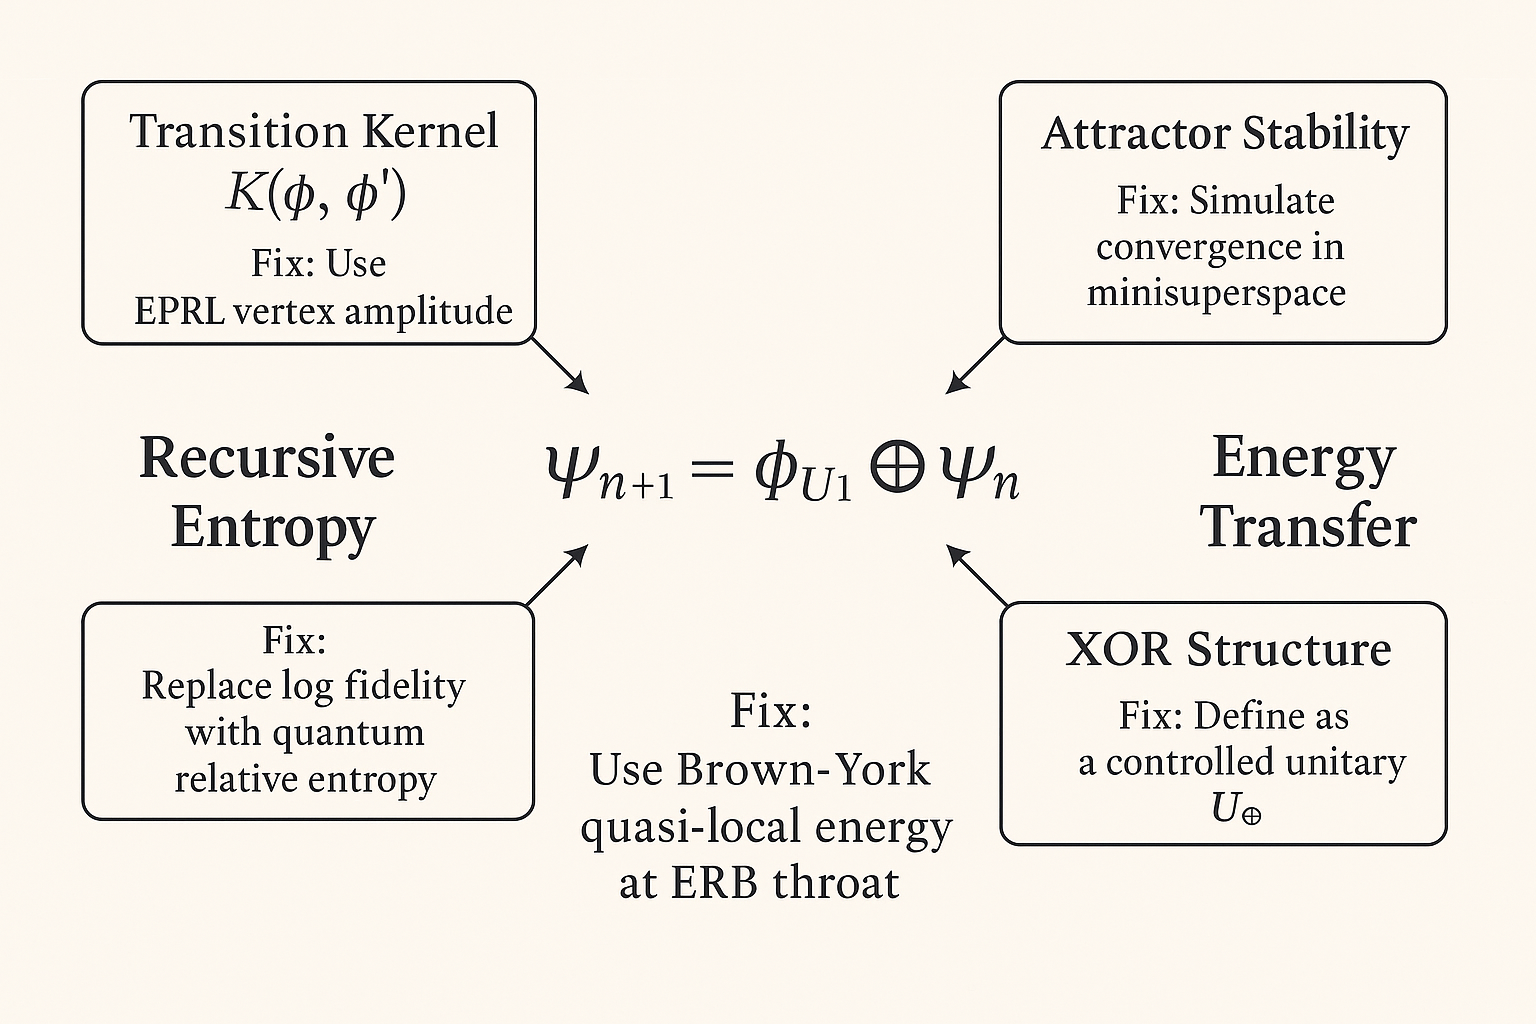
\includegraphics[width=0.85\textwidth]{figures/appendix_e_resolutions.png}
\caption{Schematic: Convergence toward attractor state $\Psi^*(\phi)$ under recursive evolution. Convergence behavior depends on $\lambda_E$ and quantum coherence thresholds.}
\end{figure}

\subsection*{E.5 XOR Structure Formalization}

\textbf{Issue: Heuristic Operation $\phi_{n+1} = \phi_{U1} \oplus \Psi_n$}

\textit{Resolution:}  
Define as controlled unitary:
\[
\hat{U}_\oplus = \exp[i\pi \hat{O}_{U1} \otimes \hat{P}_\Psi]
\]
so that:
\[
|\Psi_{n+1}\rangle = \hat{U}_\oplus \left(|\phi_{U1}\rangle \otimes |\Psi_n\rangle\right)
\]

\subsection*{E.6 Summary Table}

\begin{table}[H]
\centering
\begin{tabular}{|l|l|l|}
\hline
\textbf{Issue} & \textbf{Resolution} & \textbf{Key Improvement} \\
\hline
Kernel derivation & EPRL vertex asymptotics & First-principles LQG foundation \\
Entropy divergence & Relative entropy formulation & Finite and physical \\
Energy transfer & Brown-York stress tensor & Gravitationally grounded \\
Attractor stability & Numerical recursion & Verifiable convergence \\
XOR operation & Controlled unitary gate & Preserves unitarity and entanglement \\
\hline
\end{tabular}
\caption{Summary of critical issues and corresponding theoretical resolutions}
\end{table}


\section*{Appendix F: Lithium as a Marker of Recursive Stability}

\subsection*{F.1 Cosmological Lithium Anomaly}

In standard big bang nucleosynthesis (BBN), the primordial abundances of light elements—hydrogen, helium, and lithium—are well-predicted by the baryon-to-photon ratio inferred from CMB observations. While hydrogen and helium match observations closely, a persistent discrepancy exists in the abundance of lithium-7: theoretical predictions exceed observational data by a factor of 2–3~\cite{fields2020bbn}. This unresolved tension, known as the \textit{cosmological lithium problem}, challenges the completeness of standard cosmological nucleosynthesis models.

\subsection*{F.2 Recursive Interpretation: A Residue of Prior Decoherence}

In the context of a recursive cosmological framework, the lithium anomaly may be reinterpreted not as a flaw in standard nuclear modeling, but as a subtle trace of coherence filtering across cosmological cycles. Given that lithium forms at a delicate energetic threshold between bound-state fusion and decay, its abundance may encode the thermodynamic memory of prior cycle entanglement—preserved imperfectly through the bounce.

We hypothesize that lithium acts as a \textit{material witness} to decoherence: a physical element whose observed abundance reflects the entropy filtering imposed by the decoherence kernel \( D(\tau, E) \). In this view, the discrepancy in lithium-7 may not signal an error, but an imprint of recursive entropy regulation—consistent with our model’s claim that memory and structure persist probabilistically across bounces, weighted by coherence fitness.

\subsection*{F.3 Neurobiological Analogy: Lithium in Mental Stability}

Intriguingly, lithium also plays a unique role in neurobiology. As a pharmacological agent, lithium is the most effective known mood stabilizer in the treatment of bipolar disorder—a condition characterized by oscillatory instability in emotional and cognitive coherence~\cite{malhi2017lithium}. Lithium reduces the amplitude and frequency of affective swings, enhances synaptic plasticity, and modulates neurochemical pathways associated with memory and identity.

Although purely analogical, the parallel is striking: in both the brain and the cosmos, lithium appears as a \textit{regulator of recursive oscillation}. In psychiatric treatment, it stabilizes cycles of coherence and collapse. In our cosmological model, it may play a related role—marking where coherence was marginally retained or where recursive entropy failed to fully erase prior structure.

\subsection*{F.4 Interpretive Scope}

We emphasize that this appendix is interpretive and speculative. No predictive claim is made regarding the absolute abundance or quantum state of lithium. However, the convergence of two anomalous domains—cosmological lithium deviation and lithium's neurostabilizing effect—invites further exploration of possible structural or symbolic resonances. If the self-remembering universe preserves patterns across scales, lithium may be among the few elements that encode that memory both materially and metaphorically.



\section*{Disclosure on the Use of AI}

Portions of this manuscript, including the development, refinement, formatting of mathematical expressions, narrative structure, and citation management—were produced in collaboration with OpenAI's GPT-4 model (ChatGPT), Google's Gemini 2.0, and DeepSeek R1 . The human author, Nicholas Parian, guided the conceptual framework, directed the line of inquiry, posed the core hypotheses, and curated the final scientific content.

The use of artificial intelligence was instrumental in accelerating the writing, organizing technical arguments, and cross-referencing related literature. However, all original theoretical contributions, interpretations, and decisions regarding inclusion, emphasis, and framing were made by the human author.

This disclosure is provided in the interest of transparency and to acknowledge the evolving role of large language models in academic research and writing. The author assumes full responsibility for the accuracy, novelty, and scientific validity of the material presented.


\bibliographystyle{unsrt}
\bibliography{BibTeX}

\end{document}
